%% Run LaTeX on this file several times to get Table of Contents,
%% cross-references, and citations.

\documentclass[11pt]{book}
\usepackage{gvv}
\usepackage{gvv-book-bkup}
%\usepackage{Wiley-AuthoringTemplate}
\usepackage[sectionbib,authoryear]{natbib}% for name-date citation comment the below line
%\usepackage[sectionbib,numbers]{natbib}% for numbered citation comment the above line

%%********************************************************************%%
%%       How many levels of section head would you like numbered?     %%
%% 0= no section numbers, 1= section, 2= subsection, 3= subsubsection %%
\setcounter{secnumdepth}{3}
%%********************************************************************%%
%%**********************************************************************%%
%%     How many levels of section head would you like to appear in the  %%
%%				Table of Contents?			%%
%% 0= chapter, 1= section, 2= subsection, 3= subsubsection titles.	%%
\setcounter{tocdepth}{2}
%%**********************************************************************%%
\setcounter{tocdepth}{3}
%\includeonly{ch01}
\makeindex

\begin{document}

\frontmatter
%%%%%%%%%%%%%%%%%%%%%%%%%%%%%%%%%%%%%%%%%%%%%%%%%%%%%%%%%%%%%%%%
%% Title Pages
%% Wiley will provide title and copyright page, but you can make
%% your own titlepages if you'd like anyway
%% Setting up title pages, type in the appropriate names here:

\booktitle{CBSE Math}

\subtitle{Made Simple}

\AuAff{G. V. V. Sharma}

%% \\ will start a new line.
%% You may add \affil{} for affiliation, ie,
%\authors{Robert M. Groves\\
%\affil{Universitat de les Illes Balears}
%Floyd J. Fowler, Jr.\\
%\affil{University of New Mexico}
%}

%% Print Half Title and Title Page:
%\halftitlepage
\titlepage

%%%%%%%%%%%%%%%%%%%%%%%%%%%%%%%%%%%%%%%%%%%%%%%%%%%%%%%%%%%%%%%%
%%Copyright Page

\begin{copyrightpage}{2023}
%Title, etc
\end{copyrightpage}

% Note, you must use \ to start indented lines, ie,
% 
% \begin{copyrightpage}{2004}
% Survey Methodology / Robert M. Groves . . . [et al.].
% \       p. cm.---(Wiley series in survey methodology)
% \    ``Wiley-Interscience."
% \    Includes bibliographical references and index.
% \    ISBN 0-471-48348-6 (pbk.)
% \    1. Surveys---Methodology.  2. Social 
% \  sciences---Research---Statistical methods.  I. Groves, Robert M.  II. %
% Series.\\

% HA31.2.S873 2004
% 001.4'33---dc22                                             2004044064
% \end{copyrightpage}

%%%%%%%%%%%%%%%%%%%%%%%%%%%%%%%%%%%%%%%%%%%%%%%%%%%%%%%%%%%%%%%%
%% Only Dedication (optional) 

%\dedication{To my parents}

\tableofcontents

%\listoffigures %optional
%\listoftables  %optional

%% or Contributor Page for edited books
%% before \tableofcontents

%%%%%%%%%%%%%%%%%%%%%%%%%%%%%%%%%%%%%%%%%%%%%%%%%%%%%%%%%%%%%%%%
%  Contributors Page for Edited Book
%%%%%%%%%%%%%%%%%%%%%%%%%%%%%%%%%%%%%%%%%%%%%%%%%%%%%%%%%%%%%%%%

% If your book has chapters written by different authors,
% you'll need a Contributors page.

% Use \begin{contributors}...\end{contributors} and
% then enter each author with the \name{} command, followed
% by the affiliation information.

% \begin{contributors}
% \name{Masayki Abe,} Fujitsu Laboratories Ltd., Fujitsu Limited, Atsugi, Japan
%
% \name{L. A. Akers,} Center for Solid State Electronics Research, Arizona State University, Tempe, Arizona
%
% \name{G. H. Bernstein,} Department of Electrical and Computer Engineering, University of Notre Dame, Notre Dame, South Bend, Indiana; formerly of
% Center for Solid State Electronics Research, Arizona
% State University, Tempe, Arizona 
% \end{contributors}

%%%%%%%%%%%%%%%%%%%%%%%%%%%%%%%%%%%%%%%%%%%%%%%%%%%%%%%%%%%%%%%%
% Optional Foreword:

%\begin{foreword}
%\lipsum[1-2]
%\end{foreword}

%%%%%%%%%%%%%%%%%%%%%%%%%%%%%%%%%%%%%%%%%%%%%%%%%%%%%%%%%%%%%%%%
% Optional Preface:

%\begin{preface}
%\lipsum[1-1]
%\prefaceauthor{}
%\where{place\\
% date}
%\end{preface}

% ie,
% \begin{preface}
% This is an example preface.
% \prefaceauthor{R. K. Watts}
% \where{Durham, North Carolina\\
% September, 2004}

%%%%%%%%%%%%%%%%%%%%%%%%%%%%%%%%%%%%%%%%%%%%%%%%%%%%%%%%%%%%%%%%
% Optional Acknowledgments:

%\acknowledgments
%\lipsum[1-2]
%\authorinitials{I. R. S.}  

%%%%%%%%%%%%%%%%%%%%%%%%%%%%%%%%
%% Glossary Type of Environment:

% \begin{glossary}
% \term{<term>}{<description>}
% \end{glossary}

%%%%%%%%%%%%%%%%%%%%%%%%%%%%%%%%
%\begin{acronyms}
%\acro{ASTA}{Arrivals See Time Averages}
%\acro{BHCA}{Busy Hour Call Attempts}
%\acro{BR}{Bandwidth Reservation}
%\acro{b.u.}{bandwidth unit(s)}
%\acro{CAC}{Call / Connection Admission Control}
%\acro{CBP}{Call Blocking Probability(-ies)}
%\acro{CCS}{Centum Call Seconds}
%\acro{CDTM}{Connection Dependent Threshold Model}
%\acro{CS}{Complete Sharing}
%\acro{DiffServ}{Differentiated Services}
%\acro{EMLM}{Erlang Multirate Loss Model}
%\acro{erl}{The Erlang unit of traffic-load}
%\acro{FIFO}{First in - First out}
%\acro{GB}{Global balance}
%\acro{GoS}{Grade of Service}
%\acro{ICT}{Information and Communication Technology}
%\acro{IntServ}{Integrated Services}
%\acro{IP}{Internet Protocol}
%\acro{ITU-T}{International Telecommunication Unit -- Standardization sector}
%\acro{LB}{Local balance}
%\acro{LHS}{Left hand side}
%\acro{LIFO}{Last in - First out}
%\acro{MMPP}{Markov Modulated Poisson Process}
%\acro{MPLS}{Multiple Protocol Labeling Switching}
%\acro{MRM}{Multi-Retry Model}
%\acro{MTM}{Multi-Threshold Model}
%\acro{PASTA}{Poisson Arrivals See Time Averages}
%\acro{PDF}{Probability Distribution Function}
%\acro{pdf}{probability density function}
%\acro{PFS}{Product Form Solution}
%\acro{QoS}{Quality of Service}
%\acro{r.v.}{random variable(s)}
%\acro{RED}{random early detection}
%\acro{RHS}{Right hand side}
%\acro{RLA}{Reduced Load Approximation}
%\acro{SIRO}{service in random order}
%\acro{SRM}{Single-Retry Model}
%\acro{STM}{Single-Threshold Model}
%\acro{TCP}{Transport Control Protocol}
%\acro{TH}{Threshold(s)}
%\acro{UDP}{User Datagram Protocol}
%\end{acronyms}

\setcounter{page}{1}

\begin{introduction}
This book links high school coordinate geometry to linear algebra and matrix analysis through solved problems.

\end{introduction}

\mainmatter
\chapter{Vectors}
\section{2020}
\subsection{10}
\input{2020/vetors1.0.tex}
\subsection{12}
\input{2020/vetors2.0.tex}
\section{2023}
\subsection{10}
\input{2023/vectors10-1.tex}
\input{2023/Vectors.tex}
\subsection{12}
\input{2023/vector12-1.tex}
\section{2022}
\subsection{10}
\input{2022/maths1.tex}
\subsection{12}
\begin{enumerate}
\item $\overrightarrow{a}$   and  $\overrightarrow{ b}$ are two unit vectors such that \begin{align} \abs { 2\overrightarrow{ a}+3\overrightarrow{ b}} = \abs{3\overrightarrow{ a} - 2\overrightarrow{ b}}. \end{align} Find the angle between $\overrightarrow{ a }$ and $\overrightarrow{ b }$.
\item If $\overrightarrow{ a}$  and $\overrightarrow{b}$ are two vectors such that  \begin{align}\overrightarrow{a} = \hat{i} - \hat{j} + \hat{k} \end{align}and  \begin{align}\overrightarrow{b} = 2\hat{i} - \hat{j} - 3\hat{k}\end{align} then find the vector $\overrightarrow{c}$, given that \begin{align}\overrightarrow{a} \times \overrightarrow{c} = \overrightarrow{b}\end{align}  and \begin{align}\overrightarrow{a}.\overrightarrow{c}= 4.\end{align}
\item If \begin{align} \abs{\overrightarrow{ a } \times \overrightarrow { b }}^2 + \abs { \overrightarrow{ a } . \overrightarrow{ b }}^2= 400 \end{align} and  \begin{align}\abs { \overrightarrow{ b}} = 5 \end{align} find the value of  $\abs{\overrightarrow{ a }}$. 
\item If \begin{align}\overrightarrow{a} = \hat{i} + \hat{ j} + \hat{ k} , \overrightarrow{a} . \overrightarrow{b} = 1\end{align}  and \begin{align}\overrightarrow{a} \times \overrightarrow{b} = \hat{j} - \hat{k}\end{align},  then find  $\abs{\overrightarrow{b}}$ 
\item If \begin{align}\abs{\overrightarrow{ a}}= 3, \abs{\overrightarrow{ b}} = 2\sqrt{ 3}\end{align}  and \begin{align}\overrightarrow{ a} . \overrightarrow{ b} = 6,\end{align}then find the value of $\abs{\overrightarrow{ a} \times \overrightarrow{ b}}$.
\item $\abs{\overrightarrow{a}} = 8, \abs{\overrightarrow{ b}} = 3$ and $\overrightarrow{a} . \overrightarrow{b} = 12\sqrt{3}$, then the value of  $\abs{\overrightarrow{a} \times \overrightarrow{b}}$ is
\begin{enumerate}                                      
\item  24                                              
\item  144                                             
\item  2                                              
\item  12                                             
\end{enumerate}
\item If$\space$ \begin{align}\overrightarrow{ a} = 2\hat{i} + \hat{j} + 3\hat{k}, \hat{b} = -\hat{i} + 2\hat{j} + \hat{k}\end{align} and \begin{align}\overrightarrow{c} = 3\hat{i} + \hat{j} + 2\hat{k}\end{align}, then find $\overrightarrow{a} . (\overrightarrow{ b} \times \overrightarrow{c})$. 
	\item $\overrightarrow{a}, \overrightarrow{ b },\overrightarrow{ c }$  and  $\overrightarrow{ d }$ are four non-zeros vectors such that  \begin{align}\overrightarrow{a}\times \overrightarrow{b}= \overrightarrow{c} \times \overrightarrow{d}\end{align}  and  \begin{align}\overrightarrow{a} \times \overrightarrow{c} = 4\overrightarrow{b} \times \overrightarrow{d}\end{align}, then show that  $(\overrightarrow{ a}-2\overrightarrow{d})$ \text{ is parallel to} $(2\overrightarrow{b}-\overrightarrow{c})$ where \begin{align}\overrightarrow{a} \neq 2\overrightarrow{d}, \overrightarrow{c} \neq 2\overrightarrow{b}\end{align}
\item If \begin{align}\overrightarrow{a} = \hat{i} + \hat{ j} + \hat{ k} , \overrightarrow{a} . \overrightarrow{b} = 1\end{align}  and \begin{align}\overrightarrow{a} \times \overrightarrow{b} = \hat{j} - \hat{k},\end{align}  then find  $\abs{\overrightarrow{b}}$
\item  If $\overrightarrow{ a}$  and  $\overrightarrow{b}$  are two vectors such that \begin{align}\abs{\overrightarrow{a} + \overrightarrow{b}} = \abs{ \overrightarrow{b}},\end{align}then prove that $(\overrightarrow{a} + 2\overrightarrow{b})$  is perpendicular to $\overrightarrow{ a}$.
\item If $\overrightarrow{ a}$ and $\overrightarrow{ b}$ are unit vectors and $\theta$ is the angle between them , then prove that sin \begin{align}\frac{\theta}{ 2} = \frac{1}{2}\abs{\overrightarrow{ a} - \overrightarrow{ b}}\end{align}
\item If $\overrightarrow{a}$ and $\overrightarrow{b}$  are two unit vectors such that and $\theta$ is the angle between them, then prove that                       \begin{align}sin \dfrac{ \theta}{2} = \frac{1}{2} \abs{\overrightarrow{a} - \overrightarrow{b}} \end{align} 
\item If \begin{align}\overrightarrow{a} = 2\hat{i} + y\hat{j} + \hat{ k}\end{align} and \begin{align}\overrightarrow{ b} = \hat{i} + 2\hat{j}+ 3\hat{k}\end{align} are two vectors for which the vector $(\overrightarrow{a}+\overrightarrow{b})$ is perpendicular to the vector  $(\overrightarrow{a}-\overrightarrow{b})$ then find all the possible values of y.
\item Write the projection of the vector $(\overrightarrow{b}+\overrightarrow{c})$  on the vector  $\overrightarrow{a}$ ,  where \begin{align}\overrightarrow{ a} = 2\hat{i}-2\hat{j}+\hat{k}, \overrightarrow{b} = \hat{i}+2\hat{j}-2\hat{k}\end{align} and \begin{align}\overrightarrow{c} = 2\hat{i}-\hat{j}+4\hat{k}.\end{align}
\item If \begin{align}\overrightarrow{ a } = 2\hat{i} - \hat{ j } +\hat{ k }, \overrightarrow{ b } = \hat{ i } + \hat{ j} - 2\hat{ k }\end{align} and  \begin{align}\overrightarrow{ c } = \hat{ i } +3\hat{j} - \hat{k}\end{align} and the projection of vector   $\overrightarrow{c} + \lambda \overrightarrow{b}$  on  vector  $\overrightarrow{a}$  is $2\sqrt{6}$, find the value of $\lambda$.
	\item If \begin{align}\overrightarrow{ a} = 2\hat{i} + \hat {j} +3\hat{k}, \hat{b} = -\hat{i} + 2\hat{j} + \hat{k }\end{align} and  \begin{align}\overrightarrow{c} = 3\hat{i} + \hat{j} + 2\hat{k}\end{align}, then find $\overrightarrow{a} . (\overrightarrow{ b} \times \overrightarrow{c})$.
\item If $\space$  \begin{align}\overrightarrow { a} = 2\hat{i} - \hat{j} + 2\hat{k}\end{align} and \begin{align}\overrightarrow{ b } = 5\hat{ i } -3\hat{j} -4\hat{k}\end{align}, then find the ratio $\dfrac{ projection  of vector\space \overrightarrow{ a }\space on vector \overrightarrow{ b }}{projection of vector \space \overrightarrow{ b }\space on  vector\space \overrightarrow{ a }}$	
	\item Show that the three vectors $2\hat{ i} - \hat{j}  + \hat{k} , \hat{i} - 3\hat{j} - 5\hat{k}$ , and $3\hat{i} - 4\hat{j} - 4\hat{k}$ form the vertices of a right-angled triangle. If \begin{align}\overrightarrow{ a} = 2\hat{i} + 2\hat{j} + 3\hat{k }, \overrightarrow{ b} = -\hat{i} + 2\hat{j} + \hat{ k }\end{align}  and  \begin{align}\overrightarrow{ c} = 3\hat{i} + \hat{ j}\end{align} are such that the vector  $(\overrightarrow{ a} + \lambda \overrightarrow{ b})$ is perpendicular to vector $\overrightarrow{ c}$, then find the value of $\lambda$.	
\item If $\overrightarrow{a} , \overrightarrow{b}$ and  $\overrightarrow{c}$ are the position vectors of the points $\vec{A}(2, 3, -4)$, $\vec{B}(3, -4, -5)$ and $\vec{C}(3, 2,-3)$ and respectively, then $\abs{\overrightarrow{a} + \overrightarrow{b} + \overrightarrow{c}}$ is equal to              
\begin{enumerate}                                     
\item $\sqrt{113}$                                     
\item $\sqrt{185}$                                     
\item $\sqrt{203}$                                     
\item $\sqrt{209}$                                    
\end{enumerate}

\item Find the values $\lambda$, for which the distance of point $( 2,1, \lambda)$ from plane \begin{align}3x+5y+4z=11\end{align} is $2\sqrt{2}$ units.                            
\item Find the coordinates of the point where the line through $(3,4,1)$ crosses the ZX-plane
\item Using vectors, find the area of the triangle withvertices $\vec{A}(-1, 0, -2)$, $\vec{B}(0, 2, 1)$ and $\vec{C}(-1, 4,1)$ 
\item Using integration, find the area of triangle region whose vertices are $(2,0)$ , $(4,5)$ and $(1,4)$.
\item  If a line makes $60\degree$  and $45\degree$ angles with the positive directions of X-axis and z-axis respectively, then find the angle that it makes with the positive direction of y-axis. Hence, write the direction cosines of the line.
\item The Cartesian equation of a line $AB$ is :         \begin{align}\frac{2x-1}{12} = \frac{ y+2}{2} = \dfrac{z-3}{3}\end{align}.                        
\item Find the directions cosines of a line parallel to line $AB$.                                             
\item Find the direction cosines of a line whose cartesian equation is given as \begin{align}3x + 1 = 6y - 2 = 1 - z.\end{align}  
\item A vector of magnitude $9$ units in the direction of the vector $-2\hat{i} - \hat{j} + 2\hat{k}$ is \underline{\hspace{1cm}}
\item The two adajacent sides of a parallelogram are represented by $2\hat{i}-4\hat{j}-5\hat{k}$ and $\hat{ i}+2\hat{j}+3\hat{k}$. Find the unit vectors parallel to its diagonals. Using the diagonal vectors, find the area of the parallelogram also.                           
\item The two adjacent sides of a parallelogram are represented by vectors $2\hat{i} - 4\hat{j} + 5\hat{k}$  and  $\hat{ i} - 2\hat{j} - 3\hat{k}$. Find the unit vector parallel to one of its diagonals. Also,find the area of the parallelogram.                               
\item If $\space$ \begin{align}\overrightarrow{ a} = \overrightarrow{i} + 2\overrightarrow{j} + 3\overrightarrow{k}\end{align}   and \begin{align}\overrightarrow{ b} = 2\hat{i} + 4\hat{j} - 5\hat{k}\end{align} represent two adjacent sides of a parallelogram, then find the unit vector parallel to the diagonal of the parallelogram. 
\item Unit vector along $\overrightarrow{PQ}$, where coordinates of P and Q respectively are (2,1,-1) and (4,4,-7) is
\begin{enumerate}
\item $ 2\hat i+3\hat j-6\hat k $
\item $ -2\hat i-3\hat j+6\hat k $
\item $ -\frac{2}{7}\hat i-\frac{3}{7}\hat j+\frac{6}{7}\hat k $
\item $ \frac{2}{7}\hat i+\frac{3}{7}\hat j-\frac{6}{7}\hat k $
\end{enumerate}
\item If in $\triangle ABC$, $\overrightarrow{BA}=2\vec a$ and $\overrightarrow{BC}=3\vec b$,then $\overrightarrow{AC}$ is
\begin{enumerate}
\item $ 2\vec a+3\vec b $
\item $ 2\vec a-3\vec b $
\item $  -2\vec a+3\vec b $
\item $  -2\vec a-3\vec b $
\end{enumerate}
\item If $|\vec a \times \vec b|=\sqrt{3} $ and $\vec a \cdot \vec b =-3$, the angle between $\vec a$ and $\vec b$ is
\begin{enumerate}
\item $ \frac{2\pi}{3} $
\item $  \frac{\pi}{6} $
\item $  \frac{\pi}{3} $
\item $ \frac{5\pi}{6} $
\end{enumerate}
\item If $\vec a, \vec b, \vec c$ are three non-zero unequal vectors such that $\vec a \cdot \vec b =\vec a \cdot \vec c$, then find the angle between $\vec a$ and $\vec b - \vec c$.
     \item \textbf{Assertion(A):} If a line makes angles $\alpha, \beta, \gamma$ with positive direction of the coordinate axes, then $\sin^2 \alpha + \sin^2 \beta + \sin^2 \gamma = 2$.\\
\textbf{Reason(R):} The sum of the squares of direction cosines of a line is 1.
\end{enumerate}



\section{2021}
\subsection{10}
\input{2021/Vectors-10.tex}
\subsection{12}
\input{2021/vectors21-12.tex}
\section{2019}
\subsection{12}
\input{2019/vectors_19.tex}
\input{2019/vect55.tex}
\input{2019/vect202.tex}
\input{2019/vect19d.tex}
\input{2019/vect203.tex}
\section{2019}
\subsection{10}
\input{2019/vecj.tex}
\section{2018}
\subsection{10}
\input{2018/vectors-CBSE.tex}
\input{2018/vec22.tex}
\subsection{12}
\input{2018/vech.tex}
\input{2018/vec6.tex}
\input{2018/vec8.tex}

\section{2017}
\subsection{10}
\input{2017/vec1.tex}
\subsection{12}
\input{2017/vec17.tex}







\section{2016}
\subsection{10}
\input{2016/vector_10.tex}
\subsection{12}
\input{2016/vector.tex}
\input{2016/VECT53.tex}

\section{2015}
\subsection{10}
\input{2015/vec5.tex}
\subsection{12}
\input{2015/vector.tex}
\section{2012}
\subsection{10}
\begin{enumerate}
\item $\overrightarrow{a}$   and  $\overrightarrow{ b}$ are two unit vectors such that \begin{align} \abs { 2\overrightarrow{ a}+3\overrightarrow{ b}} = \abs{3\overrightarrow{ a} - 2\overrightarrow{ b}}. \end{align} Find the angle between $\overrightarrow{ a }$ and $\overrightarrow{ b }$.
\item If $\overrightarrow{ a}$  and $\overrightarrow{b}$ are two vectors such that  \begin{align}\overrightarrow{a} = \hat{i} - \hat{j} + \hat{k} \end{align}and  \begin{align}\overrightarrow{b} = 2\hat{i} - \hat{j} - 3\hat{k}\end{align} then find the vector $\overrightarrow{c}$, given that \begin{align}\overrightarrow{a} \times \overrightarrow{c} = \overrightarrow{b}\end{align}  and \begin{align}\overrightarrow{a}.\overrightarrow{c}= 4.\end{align}
\item If \begin{align} \abs{\overrightarrow{ a } \times \overrightarrow { b }}^2 + \abs { \overrightarrow{ a } . \overrightarrow{ b }}^2= 400 \end{align} and  \begin{align}\abs { \overrightarrow{ b}} = 5 \end{align} find the value of  $\abs{\overrightarrow{ a }}$. 
\item If \begin{align}\overrightarrow{a} = \hat{i} + \hat{ j} + \hat{ k} , \overrightarrow{a} . \overrightarrow{b} = 1\end{align}  and \begin{align}\overrightarrow{a} \times \overrightarrow{b} = \hat{j} - \hat{k}\end{align},  then find  $\abs{\overrightarrow{b}}$ 
\item If \begin{align}\abs{\overrightarrow{ a}}= 3, \abs{\overrightarrow{ b}} = 2\sqrt{ 3}\end{align}  and \begin{align}\overrightarrow{ a} . \overrightarrow{ b} = 6,\end{align}then find the value of $\abs{\overrightarrow{ a} \times \overrightarrow{ b}}$.
\item $\abs{\overrightarrow{a}} = 8, \abs{\overrightarrow{ b}} = 3$ and $\overrightarrow{a} . \overrightarrow{b} = 12\sqrt{3}$, then the value of  $\abs{\overrightarrow{a} \times \overrightarrow{b}}$ is
\begin{enumerate}                                      
\item  24                                              
\item  144                                             
\item  2                                              
\item  12                                             
\end{enumerate}
\item If$\space$ \begin{align}\overrightarrow{ a} = 2\hat{i} + \hat{j} + 3\hat{k}, \hat{b} = -\hat{i} + 2\hat{j} + \hat{k}\end{align} and \begin{align}\overrightarrow{c} = 3\hat{i} + \hat{j} + 2\hat{k}\end{align}, then find $\overrightarrow{a} . (\overrightarrow{ b} \times \overrightarrow{c})$. 
	\item $\overrightarrow{a}, \overrightarrow{ b },\overrightarrow{ c }$  and  $\overrightarrow{ d }$ are four non-zeros vectors such that  \begin{align}\overrightarrow{a}\times \overrightarrow{b}= \overrightarrow{c} \times \overrightarrow{d}\end{align}  and  \begin{align}\overrightarrow{a} \times \overrightarrow{c} = 4\overrightarrow{b} \times \overrightarrow{d}\end{align}, then show that  $(\overrightarrow{ a}-2\overrightarrow{d})$ \text{ is parallel to} $(2\overrightarrow{b}-\overrightarrow{c})$ where \begin{align}\overrightarrow{a} \neq 2\overrightarrow{d}, \overrightarrow{c} \neq 2\overrightarrow{b}\end{align}
\item If \begin{align}\overrightarrow{a} = \hat{i} + \hat{ j} + \hat{ k} , \overrightarrow{a} . \overrightarrow{b} = 1\end{align}  and \begin{align}\overrightarrow{a} \times \overrightarrow{b} = \hat{j} - \hat{k},\end{align}  then find  $\abs{\overrightarrow{b}}$
\item  If $\overrightarrow{ a}$  and  $\overrightarrow{b}$  are two vectors such that \begin{align}\abs{\overrightarrow{a} + \overrightarrow{b}} = \abs{ \overrightarrow{b}},\end{align}then prove that $(\overrightarrow{a} + 2\overrightarrow{b})$  is perpendicular to $\overrightarrow{ a}$.
\item If $\overrightarrow{ a}$ and $\overrightarrow{ b}$ are unit vectors and $\theta$ is the angle between them , then prove that sin \begin{align}\frac{\theta}{ 2} = \frac{1}{2}\abs{\overrightarrow{ a} - \overrightarrow{ b}}\end{align}
\item If $\overrightarrow{a}$ and $\overrightarrow{b}$  are two unit vectors such that and $\theta$ is the angle between them, then prove that                       \begin{align}sin \dfrac{ \theta}{2} = \frac{1}{2} \abs{\overrightarrow{a} - \overrightarrow{b}} \end{align} 
\item If \begin{align}\overrightarrow{a} = 2\hat{i} + y\hat{j} + \hat{ k}\end{align} and \begin{align}\overrightarrow{ b} = \hat{i} + 2\hat{j}+ 3\hat{k}\end{align} are two vectors for which the vector $(\overrightarrow{a}+\overrightarrow{b})$ is perpendicular to the vector  $(\overrightarrow{a}-\overrightarrow{b})$ then find all the possible values of y.
\item Write the projection of the vector $(\overrightarrow{b}+\overrightarrow{c})$  on the vector  $\overrightarrow{a}$ ,  where \begin{align}\overrightarrow{ a} = 2\hat{i}-2\hat{j}+\hat{k}, \overrightarrow{b} = \hat{i}+2\hat{j}-2\hat{k}\end{align} and \begin{align}\overrightarrow{c} = 2\hat{i}-\hat{j}+4\hat{k}.\end{align}
\item If \begin{align}\overrightarrow{ a } = 2\hat{i} - \hat{ j } +\hat{ k }, \overrightarrow{ b } = \hat{ i } + \hat{ j} - 2\hat{ k }\end{align} and  \begin{align}\overrightarrow{ c } = \hat{ i } +3\hat{j} - \hat{k}\end{align} and the projection of vector   $\overrightarrow{c} + \lambda \overrightarrow{b}$  on  vector  $\overrightarrow{a}$  is $2\sqrt{6}$, find the value of $\lambda$.
	\item If \begin{align}\overrightarrow{ a} = 2\hat{i} + \hat {j} +3\hat{k}, \hat{b} = -\hat{i} + 2\hat{j} + \hat{k }\end{align} and  \begin{align}\overrightarrow{c} = 3\hat{i} + \hat{j} + 2\hat{k}\end{align}, then find $\overrightarrow{a} . (\overrightarrow{ b} \times \overrightarrow{c})$.
\item If $\space$  \begin{align}\overrightarrow { a} = 2\hat{i} - \hat{j} + 2\hat{k}\end{align} and \begin{align}\overrightarrow{ b } = 5\hat{ i } -3\hat{j} -4\hat{k}\end{align}, then find the ratio $\dfrac{ projection  of vector\space \overrightarrow{ a }\space on vector \overrightarrow{ b }}{projection of vector \space \overrightarrow{ b }\space on  vector\space \overrightarrow{ a }}$	
	\item Show that the three vectors $2\hat{ i} - \hat{j}  + \hat{k} , \hat{i} - 3\hat{j} - 5\hat{k}$ , and $3\hat{i} - 4\hat{j} - 4\hat{k}$ form the vertices of a right-angled triangle. If \begin{align}\overrightarrow{ a} = 2\hat{i} + 2\hat{j} + 3\hat{k }, \overrightarrow{ b} = -\hat{i} + 2\hat{j} + \hat{ k }\end{align}  and  \begin{align}\overrightarrow{ c} = 3\hat{i} + \hat{ j}\end{align} are such that the vector  $(\overrightarrow{ a} + \lambda \overrightarrow{ b})$ is perpendicular to vector $\overrightarrow{ c}$, then find the value of $\lambda$.	
\item If $\overrightarrow{a} , \overrightarrow{b}$ and  $\overrightarrow{c}$ are the position vectors of the points $\vec{A}(2, 3, -4)$, $\vec{B}(3, -4, -5)$ and $\vec{C}(3, 2,-3)$ and respectively, then $\abs{\overrightarrow{a} + \overrightarrow{b} + \overrightarrow{c}}$ is equal to              
\begin{enumerate}                                     
\item $\sqrt{113}$                                     
\item $\sqrt{185}$                                     
\item $\sqrt{203}$                                     
\item $\sqrt{209}$                                    
\end{enumerate}

\item Find the values $\lambda$, for which the distance of point $( 2,1, \lambda)$ from plane \begin{align}3x+5y+4z=11\end{align} is $2\sqrt{2}$ units.                            
\item Find the coordinates of the point where the line through $(3,4,1)$ crosses the ZX-plane
\item Using vectors, find the area of the triangle withvertices $\vec{A}(-1, 0, -2)$, $\vec{B}(0, 2, 1)$ and $\vec{C}(-1, 4,1)$ 
\item Using integration, find the area of triangle region whose vertices are $(2,0)$ , $(4,5)$ and $(1,4)$.
\item  If a line makes $60\degree$  and $45\degree$ angles with the positive directions of X-axis and z-axis respectively, then find the angle that it makes with the positive direction of y-axis. Hence, write the direction cosines of the line.
\item The Cartesian equation of a line $AB$ is :         \begin{align}\frac{2x-1}{12} = \frac{ y+2}{2} = \dfrac{z-3}{3}\end{align}.                        
\item Find the directions cosines of a line parallel to line $AB$.                                             
\item Find the direction cosines of a line whose cartesian equation is given as \begin{align}3x + 1 = 6y - 2 = 1 - z.\end{align}  
\item A vector of magnitude $9$ units in the direction of the vector $-2\hat{i} - \hat{j} + 2\hat{k}$ is \underline{\hspace{1cm}}
\item The two adajacent sides of a parallelogram are represented by $2\hat{i}-4\hat{j}-5\hat{k}$ and $\hat{ i}+2\hat{j}+3\hat{k}$. Find the unit vectors parallel to its diagonals. Using the diagonal vectors, find the area of the parallelogram also.                           
\item The two adjacent sides of a parallelogram are represented by vectors $2\hat{i} - 4\hat{j} + 5\hat{k}$  and  $\hat{ i} - 2\hat{j} - 3\hat{k}$. Find the unit vector parallel to one of its diagonals. Also,find the area of the parallelogram.                               
\item If $\space$ \begin{align}\overrightarrow{ a} = \overrightarrow{i} + 2\overrightarrow{j} + 3\overrightarrow{k}\end{align}   and \begin{align}\overrightarrow{ b} = 2\hat{i} + 4\hat{j} - 5\hat{k}\end{align} represent two adjacent sides of a parallelogram, then find the unit vector parallel to the diagonal of the parallelogram. 
\item Unit vector along $\overrightarrow{PQ}$, where coordinates of P and Q respectively are (2,1,-1) and (4,4,-7) is
\begin{enumerate}
\item $ 2\hat i+3\hat j-6\hat k $
\item $ -2\hat i-3\hat j+6\hat k $
\item $ -\frac{2}{7}\hat i-\frac{3}{7}\hat j+\frac{6}{7}\hat k $
\item $ \frac{2}{7}\hat i+\frac{3}{7}\hat j-\frac{6}{7}\hat k $
\end{enumerate}
\item If in $\triangle ABC$, $\overrightarrow{BA}=2\vec a$ and $\overrightarrow{BC}=3\vec b$,then $\overrightarrow{AC}$ is
\begin{enumerate}
\item $ 2\vec a+3\vec b $
\item $ 2\vec a-3\vec b $
\item $  -2\vec a+3\vec b $
\item $  -2\vec a-3\vec b $
\end{enumerate}
\item If $|\vec a \times \vec b|=\sqrt{3} $ and $\vec a \cdot \vec b =-3$, the angle between $\vec a$ and $\vec b$ is
\begin{enumerate}
\item $ \frac{2\pi}{3} $
\item $  \frac{\pi}{6} $
\item $  \frac{\pi}{3} $
\item $ \frac{5\pi}{6} $
\end{enumerate}
\item If $\vec a, \vec b, \vec c$ are three non-zero unequal vectors such that $\vec a \cdot \vec b =\vec a \cdot \vec c$, then find the angle between $\vec a$ and $\vec b - \vec c$.
     \item \textbf{Assertion(A):} If a line makes angles $\alpha, \beta, \gamma$ with positive direction of the coordinate axes, then $\sin^2 \alpha + \sin^2 \beta + \sin^2 \gamma = 2$.\\
\textbf{Reason(R):} The sum of the squares of direction cosines of a line is 1.
\end{enumerate}






\chapter{Linear Forms}
\section{2023}
\subsection{10}
\input{2023/linear-10th.tex}
\subsection{12}                                                                                                  
\input{2023/linear-12th.tex}
\section{2022}
\subsection{10}
\begin{enumerate}

\item Solve the equations $x+2y=6$ and $2x-5y=12$ graphically.	

	\item Solve the following equations for $x$ and $y$ using cross-multiplication method:
		\begin{align}
			(ax-by)+(a+4b)=0\\(bx+ay)+(b-4a)=0
		\end{align}

	\item Find the co-ordinates of the point where the line $\dfrac{x-3}{-1}=\dfrac{y+4}{1}=\dfrac{z+5}{6}$ crosses the plane passing through the points $\left(\dfrac{7}{2},0,0\right),(0,7,0),(0,0,7)$.

	\item Electrical transmission wires which are laid down in winters are stretched tightly to accommodate expansion in summers.
		\begin{figure}[H]
			\centering
			\includegraphics[width=\columnwidth]{figs/txn}
			\caption{Electrical transmission wires connected to a transmission tower.}
			\label{fig:txn1}
		\end{figure}
		Two such wires in the figure \ref{fig:txn1} lie along the following lines:
		\begin{align}
			l_1 &: \dfrac{x+1}{3}=\dfrac{y-3}{-2}=\dfrac{z+2}{-1}\\
			l_2 &: \dfrac{x}{-1}=\dfrac{y-7}{3}=\dfrac{z+7}{-2}
		\end{align}
		Based on the given information, answer the following questions:
		\begin{enumerate}
			\item	Are the $l_1$ and $l_2$ coplanar? Justify your answer.
			\item    Find the point of intersection of lines $l_1$ and $l_2$.
		\end{enumerate}

	\item Write the cartesian equation of the line PQ passing through points P$(2,2,1)$ and Q$(5,1,-2)$. Hence, find the y-coordinate of the point on the line PQ whose z-coordinate is -2.

	\item Find the distance between the lines $x=\dfrac{y-1}{2}=\dfrac{z-2}{3}$ and $x+1=\dfrac{y+2}{2}=\dfrac{z-1}{3}$.
	
	\item Find the shortest distance between the following lines:
		\begin{align}
			\vec{r}&=3\hat{i}+5\hat{j}+7\hat{k}+\lambda(\hat{i}-2\hat{j}+\hat{k})\\\vec{r}&=(-\hat{i}-\hat{j}-\hat{k})+\mu(7\hat{i}-6\hat{j}+\hat{k})
		\end{align}

	\item Two motorcycles A and B are running at a speed more than the allowed speed on the road (as shown in figure \ref{fig:bike1}) represented by the following lines 
		\begin{align}
			\vec{r}&=\lambda(\hat{i}+2\hat{j}-\hat{k})\\\vec{r}&=(3\hat{i}+3\hat{j})+\mu(2\hat{i}+\hat{j}+\hat{k})
		\end{align}
		\begin{figure}[H]
			\centering
			\includegraphics[width=\columnwidth]{figs/bike}
			\caption{Two motorcycles moving along the road in a straight line.}
			\label{fig:bike1}
		\end{figure}
		Based on the following information, answer the following questions:
		\begin{enumerate}
			\item Find the shortest distance between the given lines.
			\item Find a point at which the motorcycles may collide.
		\end{enumerate}
	
	\item Find the shortest distance between the following lines
		\begin{align}
			\vec{r}&=(\lambda+1)\hat{i}+(\lambda+4)\hat{j}-(\lambda-3)\hat{k}\\\vec{r}&=(3-\mu)\hat{i}+(2\mu+2)\hat{j}+(\mu+6)\hat{k}
		\end{align}
	
	\item Find the shortest distance between the following lines and hence write whether the lines are intersecting or not.
		\begin{align}
			\dfrac{x-1}{2}=\dfrac{y+1}{3}=z, \dfrac{x+1}{5}=\dfrac{y-2}{1}, z=2
		\end{align}

		\item Find the equation of the plane passing through the points $(2,1,0),(3,-2,-2)$ and $(1,1,7)$. Also, obtain its distance from the origin.

	\item The foot of a perpendicular drawn from the point $(-2,-1,-3)$ on a plane is $(1,-3,3)$. Find the equation of the plane.

	\item Find the cartesian and the vector equation of a plane which passes through the point $(3,2,0)$ and contains the line $\dfrac{x-3}{1}=\dfrac{y-6}{5}=\dfrac{z-4}{4}$.

	\item The distance between the planes $4x-4y+2z+5=0$ and $2x-2y+z+6=0$ is

		\begin{enumerate}

			\item $\dfrac{1}{6}$
			\item $\dfrac{7}{6}$
			\item $\dfrac{11}{6}$
			\item $\dfrac{16}{6}$
		\end{enumerate}

	\item Find the equation of the plane through the line of intersection of the planes
		\begin{align}
			\vec{r}\cdot(\hat{i}+3\hat{j})+6&=0\\\vec{r}\cdot(3\hat{i}-\hat{j}-4\hat{k})&=0
		\end{align}which is at a  unit distance from the origin.

		\item If the distance of the point $(1,1,1)$ from the plane $x-y+z+\lambda=0$ is $\dfrac{5}{\sqrt{3}}$, find the value(s) of $\lambda$.

	\item Find the distance of the point $(2,3,4)$ measured along the line $\dfrac{x-4}{3}=\dfrac{y+5}{6}=\dfrac{z+1}{2}$ from the plane $3x+2y+2z+5=0$.

	\item Find the distance of the point $P(4,3,2)$ from the plane determined by the points $A(-1,6,-5),B(-5,-2,3)$ and $C(2,4,-5)$.

	\item The distance of the line
		\begin{align}
		\vec{r}=(\hat{i}-\hat{j})+\lambda(\hat{i}+5\hat{j}+\hat{k})\end{align}
		from the plane
		\begin{align}
		\vec{r}\cdot(\hat{i}-\hat{j}+4\hat{k})=5\end{align}
		is
		\begin{enumerate}
			\item $\sqrt{2}$
			\item $\dfrac{1}{\sqrt{2}}$
			\item $\dfrac{1}{3\sqrt{2}}$
			\item $\dfrac{-2}{3\sqrt{2}}$
		\end{enumerate}

	\item Find a unit vector perpendicular to each of the vectors $(\vec{a}+\vec{b})$ and $(\vec{a}-\vec{b})$ where 
	\begin{align}
		\vec{a}&=\hat{i}+\hat{j}+\hat{k}\\\vec{b}&=\hat{i}+2\hat{j}+3\hat{k}
	\end{align}

	\item Find the distance of the point $(1,-2,9)$ from the point of intersection of the line
		\begin{align}
			\vec{r}=4\hat{i}+2\hat{j}+7\hat{k}+\lambda(3\hat{i}+4\hat{j}+2\hat{k})
		\end{align}and the plane
		\begin{align}
			\vec{r}\cdot(\hat{i}-\hat{j}+\hat{k})=10.
		\end{align}

	\item Find the area bounded by the curves $y=\abs{x-1}$ and $y=1$, using integration.

	\item Find the coordinates of the point where the line through $(4,-3,-4)$ and $(3,-2,2)$ crosses the plane $2x+y+z=6$.

	\item Fit a straight line trend by the method of least squares and find the trend value for the year 2008 using the data from Table \ref{tab:LC}:
		\begin{table}[H]
			\caption{Table showing yearly trend of production of goods in lakh tonnes \label{tab:LC}}
			\input{2022/table2}
		\end{table}

  

  \item Equation of line passing through origin and making $30 \degree $, $60 \degree $, $90 \degree $ with x,y,z axes respectively is
    \begin{enumerate}
        \item $ \frac{2x}{\sqrt{3}}=\frac{y}{2}=\frac{z}{0} $
        \item $  \frac{2x}{\sqrt{3}}=\frac{2y}{1}=\frac{z}{0} $ 
        \item $ 2x=\frac{2y}{\sqrt{3}}=\frac{z}{1} $ 
        \item $  \frac{2x}{\sqrt{3}}=\frac{2y}{1}=\frac{z}{1} $ 
    
    \end{enumerate}
	  \item If the equation of a line is $ x=ay + b$, $z=cy + d$, then find the direction ratios of the line and a point on the line.
	  \item \begin{enumerate}
		    \item Find the equations of thee diagonals of the parallelogram PQRS whose verticees are $P(4, 2, 6)$, $Q(5,  -3, 1)$, $R(12, 4, 5)$ and $S(11, 9, -2)$. Use the equations to find thee point of intersetion of diagonals.
	    \item A line \textit{l} passes through point $(-1, 3, 2)$ and is perpendicular to both the lines $\frac{x}{1} = \frac{y}{2} = \frac{z}{3}$ and $\frac{x+2}{-3} = \frac{y-1}{2} = \frac{z + 1}{5}$. Find the vector equation of the line \textit{l}. Hence, obtain its distance from origin.
          \end{enumerate}
\end{enumerate}

\subsection{12}
\input{2022/LF.tex}
\section{2021}
\subsection{10}
\input{2021/linearforms.tex}
\subsection{12}
\input{2021/lin21.tex}
\section{2019}
\subsection{12}
\input{2019/linear_19.tex}
\input{2019/linearforms19d.tex}
\subsection{10}
\input{2019/linearj.tex}
\section{2018}
\subsection{12}
\input{2018/lineh.tex}  
\input{2018/linear6.tex} 

\section{2017}
\subsection{10}

\subsection{12}
\input{2017/liner17.tex}





\section{2016}
\subsection{12}
\input{2016/linear.tex}

\section{2015}
\subsection{12}
\input{2015/linear.tex}

\section{2011}
\subsection{10}
\input{2011/linear_forms_psv.tex}
\input{2011/Linearforms_ds.tex}

\chapter{Circles}
\section{2023}
\subsection{10}
\input{2023/Circle10.tex}
\section{2022}
\subsection{12}
\input{2022/tangent1.tex}
\subsection{10}
\input{2022/circles.tex}

\section{2021}
\subsection{10}
\input{2021/circle-10.tex}
\section{2020}
\subsection{10}
\input{2020/circ10.tex}
\section{2019} 
\subsection{10}
\input{2019/cirj.tex}
\section{2018} 
\subsection{10}
\input{2018/circles-CBSE.tex}
\subsection{12}
\input{2018/cirh.tex}
\section{2017}
\subsection{10}
\input{2017/cir1.tex}



\section{2016}
\subsection{10}
\input{2016/circles_10.tex}
\subsection{12}
\input{2016/cir53.tex}

\section{2015}
\subsection{10}
\input{2015/cir5.tex}



\section{2012}
\subsection{10}
\input{2012/circles.tex}

\section{2011}
\subsection{10}
\input{2011/circles_psv.tex}
\input{2011/circles_ds.tex}
\chapter{Intersection of Conics}
\section{2022}
\input{2022/chords.tex}
\section{2021}
\subsection{12}
\input{2021/con21.tex}
\section{2019}
\subsection{12}
\input{2019/intersection_19.tex}
\input{2019/inter55.tex}
\section{2018}
\subsection{12}
\input{2018/intersec6.tex}
\input{2018/intco8.tex}





\chapter{Probability}
\section{2021}
\subsection{10}
\begin{enumerate}
\item Let A and B be two events such that $P(A) = \frac{5}{8}$, $P(B) = \frac{1}{2}$ and  $P(A|B) = \frac{3}{4}$. Find the value of $P(B|A)$.
\item Two balls are drawn at random from a bag containing 2 red balls and 3 blue balls, without replacement. Let the variables X denotes the number of red balls. Find the probabillity distribution of X.
\item A card from a pack of 52 playing cards is lost. From the remaining cards, 2 cards are drawn at random without replacement, and are found to be both aces. Find the probability that lost card being an ace.
\item Probabilities of A and B solving a specific problem are $\frac{2}{3}$ and $\frac{3}{5},$ respectively. If both of them try independently to solve the problem, then find the probability that the problem is  solved.
\item A pair of dice is thrown. It is given that the sum of numbers  appearing on both dice is an even number. Find the probability that the number apprearing on at least one die is 3.
\item At the start of a cricket match, a coin is tossed and the team winning the toss has the opportunity to choose to bat or bowl. such a coin is unbaised with equal probabilities of getting head and tail \figref{fig:2022/probability/coin1} .
\begin{figure}[!ht]
\centering
\includegraphics[width=\columnwidth]{figs/coin}
\caption{Toss before the match}
\label{fig:2022/probability/coin1}
\end{figure}
\\ Based on the above information, answer the following question:
\begin{enumerate}
\item If such a coin is tossed 2 times, then find the probability distibution of numbers of tails.
\item Find the probability of getting at least one head in three tosses of such a coin.
\end{enumerate}
\item Two cards are drawn successively with replacement from a well shuffled pack of 52 cards. Find the probability distribution of the number of spade cards.
\item A pair of dice is thrown and the sum of the numbers appearing on the dice is observed to be 7. Find the probability that the number 5 has appeared on at least one die.
\item The probability that A hits the target is $\frac{1}{3}$ and the probability that B hits it, is $\frac{2}{5}.$ If both try to hit the target independently, find the probabillity that the target is hit. 
\item A shopkeeper sells three types of flower seeds A$_1$ , A$_1$ , A$_3$. They are sold in the form of a mixture, where the proportions of these seeds are  4 : 4 : 2, respectively. The germinaton rates of the three types of seeds are $45\%,$ $60\%$ and $35\%$ respectively \figref{fig:2022/probability/flowers11}.
\begin{figure}[!ht]
\centering                                  \includegraphics[width=\columnwidth]{figs/flowers}                                     
\caption{Three types of flowers}            
\label{fig:2022/probability/flowers11}                       
\end{figure}
\\ Based on  the above information :
\begin{enumerate}
\item  Calculate the probability that a randomly chosen seed will germinate.
\item  Calculate the probability  that the seed is of type $A_2$, given that a randomly choosen seed germinates.
\end{enumerate}
\item Three friends A, B and C got their photograph clicked. Find the probability that B is standing at the central position, given that A is standing at the left corner.
\item In a game of Archery, each ring of the Archery target is valued. The centremost ring is worth 10 points and rest of the rings are alloted points 9 to 1 in sequential order moving outwards.Archer A is likely to earn 10 points with a probability of 0.8 and Archer B is likely the earn 10 points with a probability of 0.9 \figref{fig:2022/probability/archery3}.
\begin{figure}[!ht]                     
\centering
\includegraphics[width=\columnwidth]{figs/archery}
\caption{centermost ring}                   
\label{fig:2022/probability/archery3}                        
\end{figure}
\\ Based on the above innformation, answer the following questions :
\begin{enumerate}
\item exactly one of them earns 10 points .
\item both of them earn 10 point.
\end{enumerate}
\item Event A and B are such that \begin{align} P(A) = \frac{1}{2},  P(B) = \frac{7}{12}\end{align} and \begin{align} P(\bar{A}\cup \bar{B}) = \frac{1}{4} \end{align}
Find whether the events  A and B are independent or not.
\item A box $B_1$ contain 1 white ball  and 3 red balls. Another box $B_2$ contains 2 white balls and 3 red balls. If one ball is drawn at random from each of the boxes $B_1$ and $B_2$, then find the probability that the two balls drawn are of the same colour.
\item Let X be random variable which assumes values $x_1$, $x_2$, $x_3$, $x_4$  such that\begin{align} 2P(X = x_1) = 3P (X = x_2) = P ( X = x_3) = 5P (X = x_4).\end{align}
\\ Find the probability distribution of X.
\item There are two boxes, namely box-I and box-II. Box-I contains  3 red and 6 black balls. Box-II contains 5 red and 5 black balls. One of the two boxes , is selected at random and a ball is drawn at random. The ball drawn is found to be red. Find the probability that this red ball comes out from box-II.
\item In a toss of three different coins, find the probability of comming up of three heads, if it is known that at least one head comes up.
\item A laboratory blood text is $98\%$ effective  in detecting a certain disease when it is fact, present. However, the text also yeilds a false positive result for $0.4\%$ of the healthy person tested. From a large population, it is given that $0.2\%$ of the population actually has the diseases.
\\Based on the above, answer the following questtion : 
\begin{enumerate}
\item one person, from the population, is taken at random and given the test. Find the probabiliy of his getting a positive test result.
\item what is the probability that the person actually has the disease, given that his test result is positive ?
\end{enumerate}
\item Two cards are drawn from a well-shuffled pack of playing cards one-by-one with replacement. The probability that the first card is a king and the second card is a queen is 
\begin{enumerate}
\item $\frac{1}{13} + \frac{1}{13}$
\item $ \frac{1}{13} \times \frac{4}{51}$
\item $\frac{4}{52} \times \frac{3}{51}$
\item $\frac{1}{13} \times \frac{1}{13}$
\end{enumerate}
\item For two events A and B if P(A) = $\frac{4}{10}, P{B} = \frac{8}{10}$ and $P(B|A)$ = $\frac{6}{10}$ then find $P( A \cup B).$
\item Bag I contain 4 red and 3 black balls. Bag II contains 3 red and 5 black balls. One of two bags is selected at random and a ball is drawn from the bag, which if found to be red. Find the probability that the ball is drawn from bag II.
\item Two cards are drawn successively without replacement from a well-shuffled pack of 52 cards. Find the probability distribution of the number of aces and hence find its mean.
\item The probability of solving a specific question independently by A and B are $\frac{1}{3}$ and $\frac{1}{5}$ respectively . If both try to solve the question independently, the probability that the question is solved is 
\begin{enumerate}
\item $\frac{7}{15}$
\item $\frac{8}{15}$
\item $\frac{2}{15}$
\item $\frac{14}{15}$
\end{enumerate}
\item A card is picked at random from a pack of 52 playing cards. Given that the picked up card is a queen, the probability of it being a queen of spades is \underline{\hspace{1cm}}.
\item A bag contains 19 tickets, numbered 1 to 19. A ticket is drawn at random and then another ticket is drawn without replacing the first one in the bag. Find the probability distribution of the number of even numbers on the ticket.
\item Find the probability distribution of the numbers of successes in two tosses of a die, when a success is defined as number greater than 5.
\item Ten cartoons are taken at random from an automatic packing machine. The mean net weight of the ten carton is 11.8 kg and standard deviation is 0.15 kg. Does the sample mean differ significantly from the intended mean of 12 kg ?
[Given that for d.f. = 9, $t_{0.05}$ = 2.26]
\item A Coin is tossed twice. The following table\ref{tab: Number of tails} shows the probability distribution of numbers of tails:
\begin{table}[!ht]
\input{./2022/tablep.tex}	
\caption{Table shows the probability distribution of numbers of tails \label{tab: Number of tails}}
\end{table}
\begin{enumerate}
\item Find the value of $K$.
\item Is the coin tossed biased or unbaised?
Justify your answer.
\end{enumerate}
\item If X is a random variable with probability distribution as given below \ref{tab:probability distribution}:
\begin{table}[!ht]
\input{2022/tableb.tex}
\caption{table shows the proability distribution \label{tab:probability distribution}}
\end{table}
\newline The value of K and the mean of the distribution respectively are 
\begin{enumerate}
\item $\frac{1}{7}, 1$
\item $\frac{1}{6}, 2$
\item $\frac{1}{6}, 1$
\item $1, \frac{1}{6}$
\end{enumerate}
\item The random variable X has a probability function P($x$) as defined below, where K is some number :
\\ \begin{align}P(X)=\begin{cases} K, & \text{if }  x=0 \\ 2K, & \text{if } x=1\\ 3K, & \text{if } x=2\\ 0, & \text{otherwise  } \end{cases}\end{align}
\\ Find:
\begin{enumerate}
\item The value of $K$.
\item $P(X<2),P(X \le 2), P(X \ge 2)$.
\end{enumerate}
\item Two rotten apples are mixed with 8 fresh apples. Find the probability distribution of number of rotten apples, if two apples are drawn at  random, one-by-one without replacement.

\item A die is thrown twice. What is the probability that 
\begin{enumerate}[label=(\roman*)]
 \item $5$ will come up at least once, and 
 \item $5$ will not come up either time ? 
\end{enumerate}

\item Let $A$ and $B$ be two events such that $P(A)=\frac{5}{8}$, $P(B)=\frac{1}{2}$ and $P(A/B)=\frac{3}{4}$. Find the value of $P(B/A)$.

\item Two balls are drawn at random from a bag containing $2$ red balls and $3$ blue balls, without replacement. Let the variable $X$ denotes the number of red balls. Find the probability distribution of $X$.

\item A card from a pack of $52$ playing cards is lost. From the remaining cards, $2$ cards are drawn at random without replacement, and are found to be both aces. Find the probability that lost card being an ace.

\item Probabilities of $A$ and $B$ solving a specific problem are $\frac{2}{3}$ and $\frac{3}{5}$, respectively. If both of them try independently to solve the problem, then 
find the probability that the problem is solved.

\item A pair of dice is thrown. It is given that the sum of numbers appearing on both dice is an even number. Find the probability that the number appearing on at least one die is $3$.

\item In \figref{fig:2022/probability/fig1.png},At the start of a cricket match, a coin is tossed and the team winning the 
toss has the opportunity to choose to bat or bowl. Such a coin is unbiased 
with equal probabilities of getting head and tail.

\begin{figure}[H]
        \centering
        \includegraphics[width=\columnwidth]{./figs/Screenshot (19).png}
        \caption{Tossing a coin}
        \label{fig:2022/probability/fig1.png}
    \end{figure}

Based on the above information, answer the following questions :
\begin{enumerate}[label=(\alph*)]
 \item  If such a coin is tossed $2$ times, then find the probability 
distribution of number of tails.
 
 \item Find the probability of getting at least one head in three tosses of 
such a coin. 
\end{enumerate}

\item Two cards are drawn successively with replacement from a well shuffled pack of $52$ cards. Find the probability distribution of the number of spade cards.

\item A pair of dice is thrown and the sum of the numbers appearing on the dice is observed to be $7$. Find the probability that the number $5$ has appeared on atleast one die.

\item In \figref{fig:2022/probability/fig2.png}, A shopkeeper sells three types of flower seeds $A1$, $A2$, $A3$. They are sold in the form of a mixture, where the proportions of these seeds are $4:4:2$, respectively. The germination rates of the three types of seeds are $45\%$, $60\%$ and $35\%$ respectively.

\begin{figure}[H]
        \centering
        \includegraphics[width=\columnwidth]{./figs/Screenshot (23).png}
        \caption{Three Types of Flower Seeds}
        \label{fig:2022/probability/fig2.png}
    \end{figure}

    Based on the above information:
    
    \begin{enumerate}[label=(\alph*)]
    
 \item Calculate the probability that a randomly chosen seed will germinate;
 
 \item Calculate the probability that the seed is of type $A2$, given that a randomly chosen seed germinates.

\end{enumerate}

\item Three friends $A$, $B$ and $C$ got their photograph clicked. Find the 
probability that $B$ is standing at the central position, given that $A$ is 
standing at the left corner. 

\item In \figref{fig:2022/probability/fig3.png} A coin is tossed twice. The following table shows the probability 
distribution of number of tails :
\begin{figure}[H]
        \centering
        \includegraphics[width=\columnwidth]{./figs/Screenshot (28).png}
        \caption{Probability Distribution of number of tails}
        \label{fig:2022/probability/fig3.png}
    \end{figure}

    \begin{enumerate}[label=(\alph*)]
    
 \item  Find the value of $K$. 
 
 \item  Is the coin tossed biased or unbiased ? Justify your answer.

\end{enumerate}

\item In \figref{fig:2022/probability/fig4.png} In a game of Archery, each ring of the Archery target is valued. The 
centre most ring is worth $10$ points and rest of the rings are allotted 
points $9$ to $1$ in sequential order moving outwards.

Archer A is likely to earn $10$ points with a probability of $0·8$ and Archer $B$ 
is likely the earn $10$ points with a probability of $0·9$.

\begin{figure}[H]
        \centering
        \includegraphics[width=\columnwidth]{./figs/Screenshot (26).png}
        \caption{Ring of the Archery Target}
        \label{fig:2022/probability/fig4.png}
    \end{figure}

Based on the above information, answer the following questions : 
If both of them hit the Archery target, then find the probability that 

\begin{enumerate}
    
 \item  exactly one of them earns $10$ points.
 
 \item  both of them earn $10$ points.

\end{enumerate}


\item 
\begin{enumerate}
    
 \item  Events $A$ and $B$ are such that
 P(A) =  $\frac{1}{2}$ , P(B) =  $\frac{7}{12}$  and $ P( \overline{A}  \cup  \overline{B} )= \frac{1}{4}$ Find whether the events $A$ and $B$ are independent or not.
 
 \item  A box $B_{1}$ contains $1$ white ball and $3$ red balls.Another box $B_{2}$ contains $2$ white balls and $3$ red balls.If one ball is drawn at random from each of the boxes $B_{1}$ and $B_{2}$ then find the probability that the two balls drawn are of the same colour.
 
\end{enumerate}

 \item There are two boxes, namely box-I and box-II. Box-I contains $3$ red and $6$ black balls. Box-II contains $5$ red and $5$ black balls. One of the two boxes, is selected at random and a ball is drawn at random. The ball drawn is found to be red. Find the probability that this red ball comes out from box-II.

\item In a toss of three different coins, find the probability of coming up of three heads, if it is known that at least one head comes up.

\item Two rotten apples are mixed with $8$ fresh apples. Find the probability distribution of number of rotten apples, if two apples are drawn at random, one-by-one without replacement.

\item A laboratory blood test is $98\%$ effective in detecting a certain 
disease when it is in fact, present. However, the test also yields 
a false positive result for $0·4\%$ of the healthy person tested. 
From a large population, it is given that 0·2$\%$ of the population 
actually has the disease. 
Based on the above, answer the following questions : 

  \begin{enumerate}
    
 \item One person, from the population, is taken at random and 
given the test. Find the probability of his getting a 
positive test result.  
 
 \item  What is the probability that the person actually has the 
disease, given that his test result is positive ?

\end{enumerate}

\item Two cards are drawn from a well-shuffled pack of playing 
cards one-by-one with replacement. The probability that the 
first card is a king and the second card is a queen is 

\begin{enumerate}
    
 \item $\frac{1}{13} + \frac{1}{13}$
 
 \item $\frac{1}{13} \times \frac{4}{51}$

 \item $\frac{4}{52} \times \frac{3}{51}$
 
 \item $\frac{1}{13} \times \frac{1}{13}$ 

\end{enumerate}

\item In \figref{fig:2022/probability/fig5.png} If $X$ is a random variable with probability distribution as given 
below :
\begin{figure}[H]
        \centering
        \includegraphics[width=\columnwidth]{./figs/Screenshot (32).png}
        \caption{Probability Distribution}
        \label{fig:2022/probability/fig5.png}
    \end{figure}

The value of $k$ and the mean of the distribution respectively 
are

 \begin{enumerate}
    
 \item  $\frac{1}{7}$,1 
 
 \item  $\frac{1}{6}$,2

 \item  $\frac{1}{6}$,1

 \item  $\frac{1}{6}$

\end{enumerate}


\item For two events $A$ and $B$ if P(A) = $\frac{4}{10}$, P(B) = $\frac{8}{10}$ and 
$ P(B \mid A)$=$\frac{6}{10}$, then find $ P(A \cup B)$.

\item Bag I contains $4$ red and $3$ black balls. Bag II contains $3$ red 
and $5$ black balls. One of the two bags is selected at random 
and a ball is drawn from the bag, which is found to be red. 
Find the probability that the ball is drawn from Bag II.

\item Two cards are drawn successively without replacement from a 
well-shuffled pack of $52$ cards. Find the probability 
distribution of the number of aces and hence find its mean.
\newpage

\item The probability of solving a specific question independently by $A$ and $B$ 
are $\frac{1}{3}$ and $\frac{1}{5}$ respectively. If both try to solve the question independently, 
the probability that the question is solved is 

\begin{enumerate}
    
 \item  $\frac{7}{15}$
 
 \item  $\frac{8}{15}$
 
 \item  $\frac{2}{15}$
 
 \item  $\frac{14}{15}$

\end{enumerate}

\item A card is picked at random from a pack of $52$ playing cards. Given that 
the picked up card is a queen, the probability of it being a queen of 
spades is ?

\item A bag contains $19$ tickets, numbered $1$ to $19$. A ticket is drawn at random 
and then another ticket is drawn without replacing the first one in the 
bag. Find the probability distribution of the number of even numbers on 
the ticket.

\item Find the probability distribution of the number of successes in two tosses 
of a die, when a success is defined as ‘‘number greater than $5$’’.

\item The random variable $X$ has a probability function $P(x)$ as defined below, 
where $k$ is some number :

\begin{align}
    p(x) = \begin{cases}
        k, & \text{if } x = 0, \\
        2k, & \text{if } x = 1, \\
        3k, & \text{if } x = 2, \\
        0, & \text{otherwise.}
    \end{cases}
\end{align}

Find :
\begin{enumerate}
 \item The value of $k$
 
 \item $P(X < 2)$, $P(X \leq 2)$, $P(X\ \geq 2)$
 
 \end{enumerate}

\item Consider the following hypothesis :

\begin {align}
H0 : \mu =  35\\
H1 : \mu \neq 35
\end{align}
A sample of $81$ items is taken whose mean is $37·5$ and the standard deviation is $5$. Test the hypothesis at $5\%$ level of significance.

[Given : Critical value of $Z$ for a two-tailed test at $5\%$ level of significance is $1.96$]

\item In \figref{fig:2022/probability/fig6.png} Fit a straight line trend by the method of least squares and find the trend 
value for the year $2008$ for the following data :

\begin{figure}[H]
        \centering
        \includegraphics[width=\columnwidth]{./figs/Screenshot (37).png}
        \caption{Years and Production}
        \label{fig:2022/probability/fig6.png}
    \end{figure}


    \item If A and B are two events such that $P(A/B)=2 \times P(B/A)$ and $P(A)+P(B)=\frac{2}{3}$, then $P(B)$ is equal to
    \begin{enumerate}
        \item $  \frac{2}{9} $
        \item $  \frac{7}{9} $ 
        \item $ \frac{4}{9} $ 
        \item $ \frac{5}{9} $ 
    \end{enumerate}
    \item \begin{enumerate}
            \item Two balls are drawn at random one by one with replacement from an urn containing equal number of red balls and green balls. Find the probability distribution of number of red balls, and also, find the mean of the random variable.
            \item A and B throw a die alternately till one of them gets a '6' and wins the game. Find the respective probabilities of winning, if A starts the game first.
        \end{enumerate}
				
\item Recent studies suggest that roughly 12\% of the world population is left handed.
\figref{fig:Fig2}
		\begin{figure}[h!]
		\centering
		  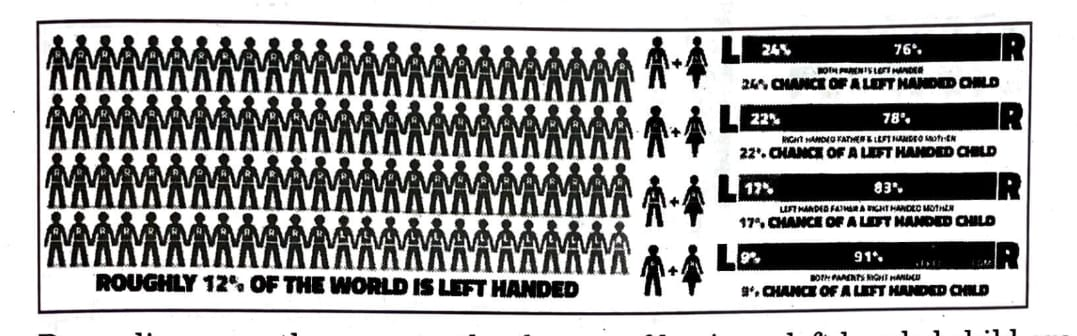
\includegraphics[height=7cm,width=11cm]{./figs/q2.png}
\caption{probability}
\end{figure}
	Depending upon the parents, the chances of having a left handed child are as follows:
		  \begin{enumerate}
                         \item : When both father and mother are left handed:\\Chances of left handed child is 24\%.
			 \item : When father is right handed and mother is left handed:\\ Chances of left handed child is 22\%.
			 \item : When father is left handed and mother is right handed:\\Chances of left handed child is 17\%.
			 \item : When both father andd mother are right handed:\\Chances of left handed child is 9\%.
		  \end{enumerate}
		  Assuming that $P(A)=P(B)=P(C)=P(D)=\frac{1}{4}$ and L denotes the event that child is left handed.\\Based on the above information, answer the following questions :
		  \begin{enumerate}
			  \item Find $P(L/C)$
			  \item Find $P(\bar L/A)$
			  \item \begin{enumerate}
					  \item Find $P(A/L)$
					  \item Find the probability that a randomly selected child is left handed given that exactly one of the parents is left handed.
			  \end{enumerate}
		  \end{enumerate}
\end{enumerate}

\subsection{12}
\input{2021/probability_cbse_21.tex}
\section{2023}
\subsection{10}
\input{2023/prob.tex}
\subsection{12}
\input{2023/probability12.tex}
\section{2022}
\subsection{10}
\input{2022/probability10.tex}
\section{2022}
\subsection{12}
\begin{enumerate}
\item Let A and B be two events such that $P(A) = \frac{5}{8}$, $P(B) = \frac{1}{2}$ and  $P(A|B) = \frac{3}{4}$. Find the value of $P(B|A)$.
\item Two balls are drawn at random from a bag containing 2 red balls and 3 blue balls, without replacement. Let the variables X denotes the number of red balls. Find the probabillity distribution of X.
\item A card from a pack of 52 playing cards is lost. From the remaining cards, 2 cards are drawn at random without replacement, and are found to be both aces. Find the probability that lost card being an ace.
\item Probabilities of A and B solving a specific problem are $\frac{2}{3}$ and $\frac{3}{5},$ respectively. If both of them try independently to solve the problem, then find the probability that the problem is  solved.
\item A pair of dice is thrown. It is given that the sum of numbers  appearing on both dice is an even number. Find the probability that the number apprearing on at least one die is 3.
\item At the start of a cricket match, a coin is tossed and the team winning the toss has the opportunity to choose to bat or bowl. such a coin is unbaised with equal probabilities of getting head and tail \figref{fig:2022/probability/coin1} .
\begin{figure}[!ht]
\centering
\includegraphics[width=\columnwidth]{figs/coin}
\caption{Toss before the match}
\label{fig:2022/probability/coin1}
\end{figure}
\\ Based on the above information, answer the following question:
\begin{enumerate}
\item If such a coin is tossed 2 times, then find the probability distibution of numbers of tails.
\item Find the probability of getting at least one head in three tosses of such a coin.
\end{enumerate}
\item Two cards are drawn successively with replacement from a well shuffled pack of 52 cards. Find the probability distribution of the number of spade cards.
\item A pair of dice is thrown and the sum of the numbers appearing on the dice is observed to be 7. Find the probability that the number 5 has appeared on at least one die.
\item The probability that A hits the target is $\frac{1}{3}$ and the probability that B hits it, is $\frac{2}{5}.$ If both try to hit the target independently, find the probabillity that the target is hit. 
\item A shopkeeper sells three types of flower seeds A$_1$ , A$_1$ , A$_3$. They are sold in the form of a mixture, where the proportions of these seeds are  4 : 4 : 2, respectively. The germinaton rates of the three types of seeds are $45\%,$ $60\%$ and $35\%$ respectively \figref{fig:2022/probability/flowers11}.
\begin{figure}[!ht]
\centering                                  \includegraphics[width=\columnwidth]{figs/flowers}                                     
\caption{Three types of flowers}            
\label{fig:2022/probability/flowers11}                       
\end{figure}
\\ Based on  the above information :
\begin{enumerate}
\item  Calculate the probability that a randomly chosen seed will germinate.
\item  Calculate the probability  that the seed is of type $A_2$, given that a randomly choosen seed germinates.
\end{enumerate}
\item Three friends A, B and C got their photograph clicked. Find the probability that B is standing at the central position, given that A is standing at the left corner.
\item In a game of Archery, each ring of the Archery target is valued. The centremost ring is worth 10 points and rest of the rings are alloted points 9 to 1 in sequential order moving outwards.Archer A is likely to earn 10 points with a probability of 0.8 and Archer B is likely the earn 10 points with a probability of 0.9 \figref{fig:2022/probability/archery3}.
\begin{figure}[!ht]                     
\centering
\includegraphics[width=\columnwidth]{figs/archery}
\caption{centermost ring}                   
\label{fig:2022/probability/archery3}                        
\end{figure}
\\ Based on the above innformation, answer the following questions :
\begin{enumerate}
\item exactly one of them earns 10 points .
\item both of them earn 10 point.
\end{enumerate}
\item Event A and B are such that \begin{align} P(A) = \frac{1}{2},  P(B) = \frac{7}{12}\end{align} and \begin{align} P(\bar{A}\cup \bar{B}) = \frac{1}{4} \end{align}
Find whether the events  A and B are independent or not.
\item A box $B_1$ contain 1 white ball  and 3 red balls. Another box $B_2$ contains 2 white balls and 3 red balls. If one ball is drawn at random from each of the boxes $B_1$ and $B_2$, then find the probability that the two balls drawn are of the same colour.
\item Let X be random variable which assumes values $x_1$, $x_2$, $x_3$, $x_4$  such that\begin{align} 2P(X = x_1) = 3P (X = x_2) = P ( X = x_3) = 5P (X = x_4).\end{align}
\\ Find the probability distribution of X.
\item There are two boxes, namely box-I and box-II. Box-I contains  3 red and 6 black balls. Box-II contains 5 red and 5 black balls. One of the two boxes , is selected at random and a ball is drawn at random. The ball drawn is found to be red. Find the probability that this red ball comes out from box-II.
\item In a toss of three different coins, find the probability of comming up of three heads, if it is known that at least one head comes up.
\item A laboratory blood text is $98\%$ effective  in detecting a certain disease when it is fact, present. However, the text also yeilds a false positive result for $0.4\%$ of the healthy person tested. From a large population, it is given that $0.2\%$ of the population actually has the diseases.
\\Based on the above, answer the following questtion : 
\begin{enumerate}
\item one person, from the population, is taken at random and given the test. Find the probabiliy of his getting a positive test result.
\item what is the probability that the person actually has the disease, given that his test result is positive ?
\end{enumerate}
\item Two cards are drawn from a well-shuffled pack of playing cards one-by-one with replacement. The probability that the first card is a king and the second card is a queen is 
\begin{enumerate}
\item $\frac{1}{13} + \frac{1}{13}$
\item $ \frac{1}{13} \times \frac{4}{51}$
\item $\frac{4}{52} \times \frac{3}{51}$
\item $\frac{1}{13} \times \frac{1}{13}$
\end{enumerate}
\item For two events A and B if P(A) = $\frac{4}{10}, P{B} = \frac{8}{10}$ and $P(B|A)$ = $\frac{6}{10}$ then find $P( A \cup B).$
\item Bag I contain 4 red and 3 black balls. Bag II contains 3 red and 5 black balls. One of two bags is selected at random and a ball is drawn from the bag, which if found to be red. Find the probability that the ball is drawn from bag II.
\item Two cards are drawn successively without replacement from a well-shuffled pack of 52 cards. Find the probability distribution of the number of aces and hence find its mean.
\item The probability of solving a specific question independently by A and B are $\frac{1}{3}$ and $\frac{1}{5}$ respectively . If both try to solve the question independently, the probability that the question is solved is 
\begin{enumerate}
\item $\frac{7}{15}$
\item $\frac{8}{15}$
\item $\frac{2}{15}$
\item $\frac{14}{15}$
\end{enumerate}
\item A card is picked at random from a pack of 52 playing cards. Given that the picked up card is a queen, the probability of it being a queen of spades is \underline{\hspace{1cm}}.
\item A bag contains 19 tickets, numbered 1 to 19. A ticket is drawn at random and then another ticket is drawn without replacing the first one in the bag. Find the probability distribution of the number of even numbers on the ticket.
\item Find the probability distribution of the numbers of successes in two tosses of a die, when a success is defined as number greater than 5.
\item Ten cartoons are taken at random from an automatic packing machine. The mean net weight of the ten carton is 11.8 kg and standard deviation is 0.15 kg. Does the sample mean differ significantly from the intended mean of 12 kg ?
[Given that for d.f. = 9, $t_{0.05}$ = 2.26]
\item A Coin is tossed twice. The following table\ref{tab: Number of tails} shows the probability distribution of numbers of tails:
\begin{table}[!ht]
\input{./2022/tablep.tex}	
\caption{Table shows the probability distribution of numbers of tails \label{tab: Number of tails}}
\end{table}
\begin{enumerate}
\item Find the value of $K$.
\item Is the coin tossed biased or unbaised?
Justify your answer.
\end{enumerate}
\item If X is a random variable with probability distribution as given below \ref{tab:probability distribution}:
\begin{table}[!ht]
\input{2022/tableb.tex}
\caption{table shows the proability distribution \label{tab:probability distribution}}
\end{table}
\newline The value of K and the mean of the distribution respectively are 
\begin{enumerate}
\item $\frac{1}{7}, 1$
\item $\frac{1}{6}, 2$
\item $\frac{1}{6}, 1$
\item $1, \frac{1}{6}$
\end{enumerate}
\item The random variable X has a probability function P($x$) as defined below, where K is some number :
\\ \begin{align}P(X)=\begin{cases} K, & \text{if }  x=0 \\ 2K, & \text{if } x=1\\ 3K, & \text{if } x=2\\ 0, & \text{otherwise  } \end{cases}\end{align}
\\ Find:
\begin{enumerate}
\item The value of $K$.
\item $P(X<2),P(X \le 2), P(X \ge 2)$.
\end{enumerate}
\item Two rotten apples are mixed with 8 fresh apples. Find the probability distribution of number of rotten apples, if two apples are drawn at  random, one-by-one without replacement.

\item A die is thrown twice. What is the probability that 
\begin{enumerate}[label=(\roman*)]
 \item $5$ will come up at least once, and 
 \item $5$ will not come up either time ? 
\end{enumerate}

\item Let $A$ and $B$ be two events such that $P(A)=\frac{5}{8}$, $P(B)=\frac{1}{2}$ and $P(A/B)=\frac{3}{4}$. Find the value of $P(B/A)$.

\item Two balls are drawn at random from a bag containing $2$ red balls and $3$ blue balls, without replacement. Let the variable $X$ denotes the number of red balls. Find the probability distribution of $X$.

\item A card from a pack of $52$ playing cards is lost. From the remaining cards, $2$ cards are drawn at random without replacement, and are found to be both aces. Find the probability that lost card being an ace.

\item Probabilities of $A$ and $B$ solving a specific problem are $\frac{2}{3}$ and $\frac{3}{5}$, respectively. If both of them try independently to solve the problem, then 
find the probability that the problem is solved.

\item A pair of dice is thrown. It is given that the sum of numbers appearing on both dice is an even number. Find the probability that the number appearing on at least one die is $3$.

\item In \figref{fig:2022/probability/fig1.png},At the start of a cricket match, a coin is tossed and the team winning the 
toss has the opportunity to choose to bat or bowl. Such a coin is unbiased 
with equal probabilities of getting head and tail.

\begin{figure}[H]
        \centering
        \includegraphics[width=\columnwidth]{./figs/Screenshot (19).png}
        \caption{Tossing a coin}
        \label{fig:2022/probability/fig1.png}
    \end{figure}

Based on the above information, answer the following questions :
\begin{enumerate}[label=(\alph*)]
 \item  If such a coin is tossed $2$ times, then find the probability 
distribution of number of tails.
 
 \item Find the probability of getting at least one head in three tosses of 
such a coin. 
\end{enumerate}

\item Two cards are drawn successively with replacement from a well shuffled pack of $52$ cards. Find the probability distribution of the number of spade cards.

\item A pair of dice is thrown and the sum of the numbers appearing on the dice is observed to be $7$. Find the probability that the number $5$ has appeared on atleast one die.

\item In \figref{fig:2022/probability/fig2.png}, A shopkeeper sells three types of flower seeds $A1$, $A2$, $A3$. They are sold in the form of a mixture, where the proportions of these seeds are $4:4:2$, respectively. The germination rates of the three types of seeds are $45\%$, $60\%$ and $35\%$ respectively.

\begin{figure}[H]
        \centering
        \includegraphics[width=\columnwidth]{./figs/Screenshot (23).png}
        \caption{Three Types of Flower Seeds}
        \label{fig:2022/probability/fig2.png}
    \end{figure}

    Based on the above information:
    
    \begin{enumerate}[label=(\alph*)]
    
 \item Calculate the probability that a randomly chosen seed will germinate;
 
 \item Calculate the probability that the seed is of type $A2$, given that a randomly chosen seed germinates.

\end{enumerate}

\item Three friends $A$, $B$ and $C$ got their photograph clicked. Find the 
probability that $B$ is standing at the central position, given that $A$ is 
standing at the left corner. 

\item In \figref{fig:2022/probability/fig3.png} A coin is tossed twice. The following table shows the probability 
distribution of number of tails :
\begin{figure}[H]
        \centering
        \includegraphics[width=\columnwidth]{./figs/Screenshot (28).png}
        \caption{Probability Distribution of number of tails}
        \label{fig:2022/probability/fig3.png}
    \end{figure}

    \begin{enumerate}[label=(\alph*)]
    
 \item  Find the value of $K$. 
 
 \item  Is the coin tossed biased or unbiased ? Justify your answer.

\end{enumerate}

\item In \figref{fig:2022/probability/fig4.png} In a game of Archery, each ring of the Archery target is valued. The 
centre most ring is worth $10$ points and rest of the rings are allotted 
points $9$ to $1$ in sequential order moving outwards.

Archer A is likely to earn $10$ points with a probability of $0·8$ and Archer $B$ 
is likely the earn $10$ points with a probability of $0·9$.

\begin{figure}[H]
        \centering
        \includegraphics[width=\columnwidth]{./figs/Screenshot (26).png}
        \caption{Ring of the Archery Target}
        \label{fig:2022/probability/fig4.png}
    \end{figure}

Based on the above information, answer the following questions : 
If both of them hit the Archery target, then find the probability that 

\begin{enumerate}
    
 \item  exactly one of them earns $10$ points.
 
 \item  both of them earn $10$ points.

\end{enumerate}


\item 
\begin{enumerate}
    
 \item  Events $A$ and $B$ are such that
 P(A) =  $\frac{1}{2}$ , P(B) =  $\frac{7}{12}$  and $ P( \overline{A}  \cup  \overline{B} )= \frac{1}{4}$ Find whether the events $A$ and $B$ are independent or not.
 
 \item  A box $B_{1}$ contains $1$ white ball and $3$ red balls.Another box $B_{2}$ contains $2$ white balls and $3$ red balls.If one ball is drawn at random from each of the boxes $B_{1}$ and $B_{2}$ then find the probability that the two balls drawn are of the same colour.
 
\end{enumerate}

 \item There are two boxes, namely box-I and box-II. Box-I contains $3$ red and $6$ black balls. Box-II contains $5$ red and $5$ black balls. One of the two boxes, is selected at random and a ball is drawn at random. The ball drawn is found to be red. Find the probability that this red ball comes out from box-II.

\item In a toss of three different coins, find the probability of coming up of three heads, if it is known that at least one head comes up.

\item Two rotten apples are mixed with $8$ fresh apples. Find the probability distribution of number of rotten apples, if two apples are drawn at random, one-by-one without replacement.

\item A laboratory blood test is $98\%$ effective in detecting a certain 
disease when it is in fact, present. However, the test also yields 
a false positive result for $0·4\%$ of the healthy person tested. 
From a large population, it is given that 0·2$\%$ of the population 
actually has the disease. 
Based on the above, answer the following questions : 

  \begin{enumerate}
    
 \item One person, from the population, is taken at random and 
given the test. Find the probability of his getting a 
positive test result.  
 
 \item  What is the probability that the person actually has the 
disease, given that his test result is positive ?

\end{enumerate}

\item Two cards are drawn from a well-shuffled pack of playing 
cards one-by-one with replacement. The probability that the 
first card is a king and the second card is a queen is 

\begin{enumerate}
    
 \item $\frac{1}{13} + \frac{1}{13}$
 
 \item $\frac{1}{13} \times \frac{4}{51}$

 \item $\frac{4}{52} \times \frac{3}{51}$
 
 \item $\frac{1}{13} \times \frac{1}{13}$ 

\end{enumerate}

\item In \figref{fig:2022/probability/fig5.png} If $X$ is a random variable with probability distribution as given 
below :
\begin{figure}[H]
        \centering
        \includegraphics[width=\columnwidth]{./figs/Screenshot (32).png}
        \caption{Probability Distribution}
        \label{fig:2022/probability/fig5.png}
    \end{figure}

The value of $k$ and the mean of the distribution respectively 
are

 \begin{enumerate}
    
 \item  $\frac{1}{7}$,1 
 
 \item  $\frac{1}{6}$,2

 \item  $\frac{1}{6}$,1

 \item  $\frac{1}{6}$

\end{enumerate}


\item For two events $A$ and $B$ if P(A) = $\frac{4}{10}$, P(B) = $\frac{8}{10}$ and 
$ P(B \mid A)$=$\frac{6}{10}$, then find $ P(A \cup B)$.

\item Bag I contains $4$ red and $3$ black balls. Bag II contains $3$ red 
and $5$ black balls. One of the two bags is selected at random 
and a ball is drawn from the bag, which is found to be red. 
Find the probability that the ball is drawn from Bag II.

\item Two cards are drawn successively without replacement from a 
well-shuffled pack of $52$ cards. Find the probability 
distribution of the number of aces and hence find its mean.
\newpage

\item The probability of solving a specific question independently by $A$ and $B$ 
are $\frac{1}{3}$ and $\frac{1}{5}$ respectively. If both try to solve the question independently, 
the probability that the question is solved is 

\begin{enumerate}
    
 \item  $\frac{7}{15}$
 
 \item  $\frac{8}{15}$
 
 \item  $\frac{2}{15}$
 
 \item  $\frac{14}{15}$

\end{enumerate}

\item A card is picked at random from a pack of $52$ playing cards. Given that 
the picked up card is a queen, the probability of it being a queen of 
spades is ?

\item A bag contains $19$ tickets, numbered $1$ to $19$. A ticket is drawn at random 
and then another ticket is drawn without replacing the first one in the 
bag. Find the probability distribution of the number of even numbers on 
the ticket.

\item Find the probability distribution of the number of successes in two tosses 
of a die, when a success is defined as ‘‘number greater than $5$’’.

\item The random variable $X$ has a probability function $P(x)$ as defined below, 
where $k$ is some number :

\begin{align}
    p(x) = \begin{cases}
        k, & \text{if } x = 0, \\
        2k, & \text{if } x = 1, \\
        3k, & \text{if } x = 2, \\
        0, & \text{otherwise.}
    \end{cases}
\end{align}

Find :
\begin{enumerate}
 \item The value of $k$
 
 \item $P(X < 2)$, $P(X \leq 2)$, $P(X\ \geq 2)$
 
 \end{enumerate}

\item Consider the following hypothesis :

\begin {align}
H0 : \mu =  35\\
H1 : \mu \neq 35
\end{align}
A sample of $81$ items is taken whose mean is $37·5$ and the standard deviation is $5$. Test the hypothesis at $5\%$ level of significance.

[Given : Critical value of $Z$ for a two-tailed test at $5\%$ level of significance is $1.96$]

\item In \figref{fig:2022/probability/fig6.png} Fit a straight line trend by the method of least squares and find the trend 
value for the year $2008$ for the following data :

\begin{figure}[H]
        \centering
        \includegraphics[width=\columnwidth]{./figs/Screenshot (37).png}
        \caption{Years and Production}
        \label{fig:2022/probability/fig6.png}
    \end{figure}


    \item If A and B are two events such that $P(A/B)=2 \times P(B/A)$ and $P(A)+P(B)=\frac{2}{3}$, then $P(B)$ is equal to
    \begin{enumerate}
        \item $  \frac{2}{9} $
        \item $  \frac{7}{9} $ 
        \item $ \frac{4}{9} $ 
        \item $ \frac{5}{9} $ 
    \end{enumerate}
    \item \begin{enumerate}
            \item Two balls are drawn at random one by one with replacement from an urn containing equal number of red balls and green balls. Find the probability distribution of number of red balls, and also, find the mean of the random variable.
            \item A and B throw a die alternately till one of them gets a '6' and wins the game. Find the respective probabilities of winning, if A starts the game first.
        \end{enumerate}
				
\item Recent studies suggest that roughly 12\% of the world population is left handed.
\figref{fig:Fig2}
		\begin{figure}[h!]
		\centering
		  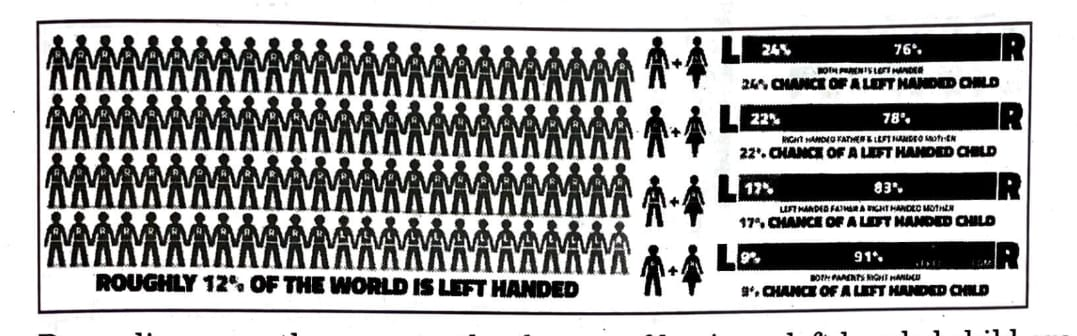
\includegraphics[height=7cm,width=11cm]{./figs/q2.png}
\caption{probability}
\end{figure}
	Depending upon the parents, the chances of having a left handed child are as follows:
		  \begin{enumerate}
                         \item : When both father and mother are left handed:\\Chances of left handed child is 24\%.
			 \item : When father is right handed and mother is left handed:\\ Chances of left handed child is 22\%.
			 \item : When father is left handed and mother is right handed:\\Chances of left handed child is 17\%.
			 \item : When both father andd mother are right handed:\\Chances of left handed child is 9\%.
		  \end{enumerate}
		  Assuming that $P(A)=P(B)=P(C)=P(D)=\frac{1}{4}$ and L denotes the event that child is left handed.\\Based on the above information, answer the following questions :
		  \begin{enumerate}
			  \item Find $P(L/C)$
			  \item Find $P(\bar L/A)$
			  \item \begin{enumerate}
					  \item Find $P(A/L)$
					  \item Find the probability that a randomly selected child is left handed given that exactly one of the parents is left handed.
			  \end{enumerate}
		  \end{enumerate}
\end{enumerate}

\section{2020}
\subsection{10}
\input{2020/prob10.tex}
\subsection{12}
\input{2020/prob12.tex}
\section{2019}
\subsection{12}
\input{2019/probab_19.tex}
\input{2019/probb55.tex}
\input{2019/prob202.tex}
\input{2019/probab19d.tex}
\input{2019/prob203.tex}
\section{2019}
\subsection{10}
\input{2019/probj.tex}
\section{2018}
\subsection{10}
\input{2018/probability-CBSE.tex}
\input{2018/prob22.tex}
\subsection{12}
\input{2018/probh.tex}
\input{2018/prob6.tex}
\input{2018/pro8.tex}

\section{2017}
\subsection{10}
\input{2017/prob1.tex}
\subsection{12}
\input{2017/prob17.tex}




\section{2016}
\subsection{10}
\input{2016/prob_10.tex}
\subsection{12}
\input{2016/prob.tex}
\input{2016/PROB53.tex}
\section{2015}
\subsection{10}
\input{2015/prob.tex}
\input{2015/prob5.tex}
\subsection{12}
\input{2015/probab.tex}
\section{2012}
\subsection{10}
\begin{enumerate}
\item Let A and B be two events such that $P(A) = \frac{5}{8}$, $P(B) = \frac{1}{2}$ and  $P(A|B) = \frac{3}{4}$. Find the value of $P(B|A)$.
\item Two balls are drawn at random from a bag containing 2 red balls and 3 blue balls, without replacement. Let the variables X denotes the number of red balls. Find the probabillity distribution of X.
\item A card from a pack of 52 playing cards is lost. From the remaining cards, 2 cards are drawn at random without replacement, and are found to be both aces. Find the probability that lost card being an ace.
\item Probabilities of A and B solving a specific problem are $\frac{2}{3}$ and $\frac{3}{5},$ respectively. If both of them try independently to solve the problem, then find the probability that the problem is  solved.
\item A pair of dice is thrown. It is given that the sum of numbers  appearing on both dice is an even number. Find the probability that the number apprearing on at least one die is 3.
\item At the start of a cricket match, a coin is tossed and the team winning the toss has the opportunity to choose to bat or bowl. such a coin is unbaised with equal probabilities of getting head and tail \figref{fig:2022/probability/coin1} .
\begin{figure}[!ht]
\centering
\includegraphics[width=\columnwidth]{figs/coin}
\caption{Toss before the match}
\label{fig:2022/probability/coin1}
\end{figure}
\\ Based on the above information, answer the following question:
\begin{enumerate}
\item If such a coin is tossed 2 times, then find the probability distibution of numbers of tails.
\item Find the probability of getting at least one head in three tosses of such a coin.
\end{enumerate}
\item Two cards are drawn successively with replacement from a well shuffled pack of 52 cards. Find the probability distribution of the number of spade cards.
\item A pair of dice is thrown and the sum of the numbers appearing on the dice is observed to be 7. Find the probability that the number 5 has appeared on at least one die.
\item The probability that A hits the target is $\frac{1}{3}$ and the probability that B hits it, is $\frac{2}{5}.$ If both try to hit the target independently, find the probabillity that the target is hit. 
\item A shopkeeper sells three types of flower seeds A$_1$ , A$_1$ , A$_3$. They are sold in the form of a mixture, where the proportions of these seeds are  4 : 4 : 2, respectively. The germinaton rates of the three types of seeds are $45\%,$ $60\%$ and $35\%$ respectively \figref{fig:2022/probability/flowers11}.
\begin{figure}[!ht]
\centering                                  \includegraphics[width=\columnwidth]{figs/flowers}                                     
\caption{Three types of flowers}            
\label{fig:2022/probability/flowers11}                       
\end{figure}
\\ Based on  the above information :
\begin{enumerate}
\item  Calculate the probability that a randomly chosen seed will germinate.
\item  Calculate the probability  that the seed is of type $A_2$, given that a randomly choosen seed germinates.
\end{enumerate}
\item Three friends A, B and C got their photograph clicked. Find the probability that B is standing at the central position, given that A is standing at the left corner.
\item In a game of Archery, each ring of the Archery target is valued. The centremost ring is worth 10 points and rest of the rings are alloted points 9 to 1 in sequential order moving outwards.Archer A is likely to earn 10 points with a probability of 0.8 and Archer B is likely the earn 10 points with a probability of 0.9 \figref{fig:2022/probability/archery3}.
\begin{figure}[!ht]                     
\centering
\includegraphics[width=\columnwidth]{figs/archery}
\caption{centermost ring}                   
\label{fig:2022/probability/archery3}                        
\end{figure}
\\ Based on the above innformation, answer the following questions :
\begin{enumerate}
\item exactly one of them earns 10 points .
\item both of them earn 10 point.
\end{enumerate}
\item Event A and B are such that \begin{align} P(A) = \frac{1}{2},  P(B) = \frac{7}{12}\end{align} and \begin{align} P(\bar{A}\cup \bar{B}) = \frac{1}{4} \end{align}
Find whether the events  A and B are independent or not.
\item A box $B_1$ contain 1 white ball  and 3 red balls. Another box $B_2$ contains 2 white balls and 3 red balls. If one ball is drawn at random from each of the boxes $B_1$ and $B_2$, then find the probability that the two balls drawn are of the same colour.
\item Let X be random variable which assumes values $x_1$, $x_2$, $x_3$, $x_4$  such that\begin{align} 2P(X = x_1) = 3P (X = x_2) = P ( X = x_3) = 5P (X = x_4).\end{align}
\\ Find the probability distribution of X.
\item There are two boxes, namely box-I and box-II. Box-I contains  3 red and 6 black balls. Box-II contains 5 red and 5 black balls. One of the two boxes , is selected at random and a ball is drawn at random. The ball drawn is found to be red. Find the probability that this red ball comes out from box-II.
\item In a toss of three different coins, find the probability of comming up of three heads, if it is known that at least one head comes up.
\item A laboratory blood text is $98\%$ effective  in detecting a certain disease when it is fact, present. However, the text also yeilds a false positive result for $0.4\%$ of the healthy person tested. From a large population, it is given that $0.2\%$ of the population actually has the diseases.
\\Based on the above, answer the following questtion : 
\begin{enumerate}
\item one person, from the population, is taken at random and given the test. Find the probabiliy of his getting a positive test result.
\item what is the probability that the person actually has the disease, given that his test result is positive ?
\end{enumerate}
\item Two cards are drawn from a well-shuffled pack of playing cards one-by-one with replacement. The probability that the first card is a king and the second card is a queen is 
\begin{enumerate}
\item $\frac{1}{13} + \frac{1}{13}$
\item $ \frac{1}{13} \times \frac{4}{51}$
\item $\frac{4}{52} \times \frac{3}{51}$
\item $\frac{1}{13} \times \frac{1}{13}$
\end{enumerate}
\item For two events A and B if P(A) = $\frac{4}{10}, P{B} = \frac{8}{10}$ and $P(B|A)$ = $\frac{6}{10}$ then find $P( A \cup B).$
\item Bag I contain 4 red and 3 black balls. Bag II contains 3 red and 5 black balls. One of two bags is selected at random and a ball is drawn from the bag, which if found to be red. Find the probability that the ball is drawn from bag II.
\item Two cards are drawn successively without replacement from a well-shuffled pack of 52 cards. Find the probability distribution of the number of aces and hence find its mean.
\item The probability of solving a specific question independently by A and B are $\frac{1}{3}$ and $\frac{1}{5}$ respectively . If both try to solve the question independently, the probability that the question is solved is 
\begin{enumerate}
\item $\frac{7}{15}$
\item $\frac{8}{15}$
\item $\frac{2}{15}$
\item $\frac{14}{15}$
\end{enumerate}
\item A card is picked at random from a pack of 52 playing cards. Given that the picked up card is a queen, the probability of it being a queen of spades is \underline{\hspace{1cm}}.
\item A bag contains 19 tickets, numbered 1 to 19. A ticket is drawn at random and then another ticket is drawn without replacing the first one in the bag. Find the probability distribution of the number of even numbers on the ticket.
\item Find the probability distribution of the numbers of successes in two tosses of a die, when a success is defined as number greater than 5.
\item Ten cartoons are taken at random from an automatic packing machine. The mean net weight of the ten carton is 11.8 kg and standard deviation is 0.15 kg. Does the sample mean differ significantly from the intended mean of 12 kg ?
[Given that for d.f. = 9, $t_{0.05}$ = 2.26]
\item A Coin is tossed twice. The following table\ref{tab: Number of tails} shows the probability distribution of numbers of tails:
\begin{table}[!ht]
\input{./2022/tablep.tex}	
\caption{Table shows the probability distribution of numbers of tails \label{tab: Number of tails}}
\end{table}
\begin{enumerate}
\item Find the value of $K$.
\item Is the coin tossed biased or unbaised?
Justify your answer.
\end{enumerate}
\item If X is a random variable with probability distribution as given below \ref{tab:probability distribution}:
\begin{table}[!ht]
\input{2022/tableb.tex}
\caption{table shows the proability distribution \label{tab:probability distribution}}
\end{table}
\newline The value of K and the mean of the distribution respectively are 
\begin{enumerate}
\item $\frac{1}{7}, 1$
\item $\frac{1}{6}, 2$
\item $\frac{1}{6}, 1$
\item $1, \frac{1}{6}$
\end{enumerate}
\item The random variable X has a probability function P($x$) as defined below, where K is some number :
\\ \begin{align}P(X)=\begin{cases} K, & \text{if }  x=0 \\ 2K, & \text{if } x=1\\ 3K, & \text{if } x=2\\ 0, & \text{otherwise  } \end{cases}\end{align}
\\ Find:
\begin{enumerate}
\item The value of $K$.
\item $P(X<2),P(X \le 2), P(X \ge 2)$.
\end{enumerate}
\item Two rotten apples are mixed with 8 fresh apples. Find the probability distribution of number of rotten apples, if two apples are drawn at  random, one-by-one without replacement.

\item A die is thrown twice. What is the probability that 
\begin{enumerate}[label=(\roman*)]
 \item $5$ will come up at least once, and 
 \item $5$ will not come up either time ? 
\end{enumerate}

\item Let $A$ and $B$ be two events such that $P(A)=\frac{5}{8}$, $P(B)=\frac{1}{2}$ and $P(A/B)=\frac{3}{4}$. Find the value of $P(B/A)$.

\item Two balls are drawn at random from a bag containing $2$ red balls and $3$ blue balls, without replacement. Let the variable $X$ denotes the number of red balls. Find the probability distribution of $X$.

\item A card from a pack of $52$ playing cards is lost. From the remaining cards, $2$ cards are drawn at random without replacement, and are found to be both aces. Find the probability that lost card being an ace.

\item Probabilities of $A$ and $B$ solving a specific problem are $\frac{2}{3}$ and $\frac{3}{5}$, respectively. If both of them try independently to solve the problem, then 
find the probability that the problem is solved.

\item A pair of dice is thrown. It is given that the sum of numbers appearing on both dice is an even number. Find the probability that the number appearing on at least one die is $3$.

\item In \figref{fig:2022/probability/fig1.png},At the start of a cricket match, a coin is tossed and the team winning the 
toss has the opportunity to choose to bat or bowl. Such a coin is unbiased 
with equal probabilities of getting head and tail.

\begin{figure}[H]
        \centering
        \includegraphics[width=\columnwidth]{./figs/Screenshot (19).png}
        \caption{Tossing a coin}
        \label{fig:2022/probability/fig1.png}
    \end{figure}

Based on the above information, answer the following questions :
\begin{enumerate}[label=(\alph*)]
 \item  If such a coin is tossed $2$ times, then find the probability 
distribution of number of tails.
 
 \item Find the probability of getting at least one head in three tosses of 
such a coin. 
\end{enumerate}

\item Two cards are drawn successively with replacement from a well shuffled pack of $52$ cards. Find the probability distribution of the number of spade cards.

\item A pair of dice is thrown and the sum of the numbers appearing on the dice is observed to be $7$. Find the probability that the number $5$ has appeared on atleast one die.

\item In \figref{fig:2022/probability/fig2.png}, A shopkeeper sells three types of flower seeds $A1$, $A2$, $A3$. They are sold in the form of a mixture, where the proportions of these seeds are $4:4:2$, respectively. The germination rates of the three types of seeds are $45\%$, $60\%$ and $35\%$ respectively.

\begin{figure}[H]
        \centering
        \includegraphics[width=\columnwidth]{./figs/Screenshot (23).png}
        \caption{Three Types of Flower Seeds}
        \label{fig:2022/probability/fig2.png}
    \end{figure}

    Based on the above information:
    
    \begin{enumerate}[label=(\alph*)]
    
 \item Calculate the probability that a randomly chosen seed will germinate;
 
 \item Calculate the probability that the seed is of type $A2$, given that a randomly chosen seed germinates.

\end{enumerate}

\item Three friends $A$, $B$ and $C$ got their photograph clicked. Find the 
probability that $B$ is standing at the central position, given that $A$ is 
standing at the left corner. 

\item In \figref{fig:2022/probability/fig3.png} A coin is tossed twice. The following table shows the probability 
distribution of number of tails :
\begin{figure}[H]
        \centering
        \includegraphics[width=\columnwidth]{./figs/Screenshot (28).png}
        \caption{Probability Distribution of number of tails}
        \label{fig:2022/probability/fig3.png}
    \end{figure}

    \begin{enumerate}[label=(\alph*)]
    
 \item  Find the value of $K$. 
 
 \item  Is the coin tossed biased or unbiased ? Justify your answer.

\end{enumerate}

\item In \figref{fig:2022/probability/fig4.png} In a game of Archery, each ring of the Archery target is valued. The 
centre most ring is worth $10$ points and rest of the rings are allotted 
points $9$ to $1$ in sequential order moving outwards.

Archer A is likely to earn $10$ points with a probability of $0·8$ and Archer $B$ 
is likely the earn $10$ points with a probability of $0·9$.

\begin{figure}[H]
        \centering
        \includegraphics[width=\columnwidth]{./figs/Screenshot (26).png}
        \caption{Ring of the Archery Target}
        \label{fig:2022/probability/fig4.png}
    \end{figure}

Based on the above information, answer the following questions : 
If both of them hit the Archery target, then find the probability that 

\begin{enumerate}
    
 \item  exactly one of them earns $10$ points.
 
 \item  both of them earn $10$ points.

\end{enumerate}


\item 
\begin{enumerate}
    
 \item  Events $A$ and $B$ are such that
 P(A) =  $\frac{1}{2}$ , P(B) =  $\frac{7}{12}$  and $ P( \overline{A}  \cup  \overline{B} )= \frac{1}{4}$ Find whether the events $A$ and $B$ are independent or not.
 
 \item  A box $B_{1}$ contains $1$ white ball and $3$ red balls.Another box $B_{2}$ contains $2$ white balls and $3$ red balls.If one ball is drawn at random from each of the boxes $B_{1}$ and $B_{2}$ then find the probability that the two balls drawn are of the same colour.
 
\end{enumerate}

 \item There are two boxes, namely box-I and box-II. Box-I contains $3$ red and $6$ black balls. Box-II contains $5$ red and $5$ black balls. One of the two boxes, is selected at random and a ball is drawn at random. The ball drawn is found to be red. Find the probability that this red ball comes out from box-II.

\item In a toss of three different coins, find the probability of coming up of three heads, if it is known that at least one head comes up.

\item Two rotten apples are mixed with $8$ fresh apples. Find the probability distribution of number of rotten apples, if two apples are drawn at random, one-by-one without replacement.

\item A laboratory blood test is $98\%$ effective in detecting a certain 
disease when it is in fact, present. However, the test also yields 
a false positive result for $0·4\%$ of the healthy person tested. 
From a large population, it is given that 0·2$\%$ of the population 
actually has the disease. 
Based on the above, answer the following questions : 

  \begin{enumerate}
    
 \item One person, from the population, is taken at random and 
given the test. Find the probability of his getting a 
positive test result.  
 
 \item  What is the probability that the person actually has the 
disease, given that his test result is positive ?

\end{enumerate}

\item Two cards are drawn from a well-shuffled pack of playing 
cards one-by-one with replacement. The probability that the 
first card is a king and the second card is a queen is 

\begin{enumerate}
    
 \item $\frac{1}{13} + \frac{1}{13}$
 
 \item $\frac{1}{13} \times \frac{4}{51}$

 \item $\frac{4}{52} \times \frac{3}{51}$
 
 \item $\frac{1}{13} \times \frac{1}{13}$ 

\end{enumerate}

\item In \figref{fig:2022/probability/fig5.png} If $X$ is a random variable with probability distribution as given 
below :
\begin{figure}[H]
        \centering
        \includegraphics[width=\columnwidth]{./figs/Screenshot (32).png}
        \caption{Probability Distribution}
        \label{fig:2022/probability/fig5.png}
    \end{figure}

The value of $k$ and the mean of the distribution respectively 
are

 \begin{enumerate}
    
 \item  $\frac{1}{7}$,1 
 
 \item  $\frac{1}{6}$,2

 \item  $\frac{1}{6}$,1

 \item  $\frac{1}{6}$

\end{enumerate}


\item For two events $A$ and $B$ if P(A) = $\frac{4}{10}$, P(B) = $\frac{8}{10}$ and 
$ P(B \mid A)$=$\frac{6}{10}$, then find $ P(A \cup B)$.

\item Bag I contains $4$ red and $3$ black balls. Bag II contains $3$ red 
and $5$ black balls. One of the two bags is selected at random 
and a ball is drawn from the bag, which is found to be red. 
Find the probability that the ball is drawn from Bag II.

\item Two cards are drawn successively without replacement from a 
well-shuffled pack of $52$ cards. Find the probability 
distribution of the number of aces and hence find its mean.
\newpage

\item The probability of solving a specific question independently by $A$ and $B$ 
are $\frac{1}{3}$ and $\frac{1}{5}$ respectively. If both try to solve the question independently, 
the probability that the question is solved is 

\begin{enumerate}
    
 \item  $\frac{7}{15}$
 
 \item  $\frac{8}{15}$
 
 \item  $\frac{2}{15}$
 
 \item  $\frac{14}{15}$

\end{enumerate}

\item A card is picked at random from a pack of $52$ playing cards. Given that 
the picked up card is a queen, the probability of it being a queen of 
spades is ?

\item A bag contains $19$ tickets, numbered $1$ to $19$. A ticket is drawn at random 
and then another ticket is drawn without replacing the first one in the 
bag. Find the probability distribution of the number of even numbers on 
the ticket.

\item Find the probability distribution of the number of successes in two tosses 
of a die, when a success is defined as ‘‘number greater than $5$’’.

\item The random variable $X$ has a probability function $P(x)$ as defined below, 
where $k$ is some number :

\begin{align}
    p(x) = \begin{cases}
        k, & \text{if } x = 0, \\
        2k, & \text{if } x = 1, \\
        3k, & \text{if } x = 2, \\
        0, & \text{otherwise.}
    \end{cases}
\end{align}

Find :
\begin{enumerate}
 \item The value of $k$
 
 \item $P(X < 2)$, $P(X \leq 2)$, $P(X\ \geq 2)$
 
 \end{enumerate}

\item Consider the following hypothesis :

\begin {align}
H0 : \mu =  35\\
H1 : \mu \neq 35
\end{align}
A sample of $81$ items is taken whose mean is $37·5$ and the standard deviation is $5$. Test the hypothesis at $5\%$ level of significance.

[Given : Critical value of $Z$ for a two-tailed test at $5\%$ level of significance is $1.96$]

\item In \figref{fig:2022/probability/fig6.png} Fit a straight line trend by the method of least squares and find the trend 
value for the year $2008$ for the following data :

\begin{figure}[H]
        \centering
        \includegraphics[width=\columnwidth]{./figs/Screenshot (37).png}
        \caption{Years and Production}
        \label{fig:2022/probability/fig6.png}
    \end{figure}


    \item If A and B are two events such that $P(A/B)=2 \times P(B/A)$ and $P(A)+P(B)=\frac{2}{3}$, then $P(B)$ is equal to
    \begin{enumerate}
        \item $  \frac{2}{9} $
        \item $  \frac{7}{9} $ 
        \item $ \frac{4}{9} $ 
        \item $ \frac{5}{9} $ 
    \end{enumerate}
    \item \begin{enumerate}
            \item Two balls are drawn at random one by one with replacement from an urn containing equal number of red balls and green balls. Find the probability distribution of number of red balls, and also, find the mean of the random variable.
            \item A and B throw a die alternately till one of them gets a '6' and wins the game. Find the respective probabilities of winning, if A starts the game first.
        \end{enumerate}
				
\item Recent studies suggest that roughly 12\% of the world population is left handed.
\figref{fig:Fig2}
		\begin{figure}[h!]
		\centering
		  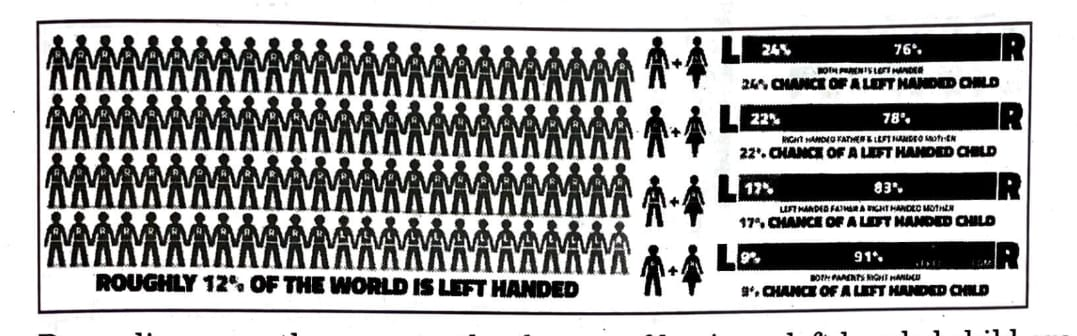
\includegraphics[height=7cm,width=11cm]{./figs/q2.png}
\caption{probability}
\end{figure}
	Depending upon the parents, the chances of having a left handed child are as follows:
		  \begin{enumerate}
                         \item : When both father and mother are left handed:\\Chances of left handed child is 24\%.
			 \item : When father is right handed and mother is left handed:\\ Chances of left handed child is 22\%.
			 \item : When father is left handed and mother is right handed:\\Chances of left handed child is 17\%.
			 \item : When both father andd mother are right handed:\\Chances of left handed child is 9\%.
		  \end{enumerate}
		  Assuming that $P(A)=P(B)=P(C)=P(D)=\frac{1}{4}$ and L denotes the event that child is left handed.\\Based on the above information, answer the following questions :
		  \begin{enumerate}
			  \item Find $P(L/C)$
			  \item Find $P(\bar L/A)$
			  \item \begin{enumerate}
					  \item Find $P(A/L)$
					  \item Find the probability that a randomly selected child is left handed given that exactly one of the parents is left handed.
			  \end{enumerate}
		  \end{enumerate}
\end{enumerate}


\section{2011}
\subsection{10}
\input{2011/probability_psv.tex}
\input{2011/probability_ds.tex}

\chapter{Construction}
\section{2023}
\subsection{10}
\input{2023/construction-10th.tex}
\section{2022}
\subsection{10}
\input{2022/construction.tex}
\section{2021}
\subsection{10}
\input{2021/construction.tex}
\section{2020}
\subsection{10}
\input{2020/cont.tex}
\section{2019} 
\subsection{10}
\input{2019/consj.tex}
\section{2018} 
\subsection{10}
\input{2018/construction-CBSE.tex}
\input{2018/con22.tex}
\section{2017}
\subsection{10}
\input{2017/cons1.tex}





\section{2016}
\subsection{10}
\input{2016/construction_10.tex}
\section{2015}
\subsection{10}
\input{2015/construction.tex}
\input{2015/con5.tex}
\section{2012}
\subsection{10}
\input{2012/construction.tex}

\section{2011}
\subsection{10}
\input{2011/construction_psv.tex}


\chapter{Optimization}
\section{2023}
\input{2023/opti.tex}
\section{2021}
\subsection{12}
\input{2022/opt_vect.tex}
\section{2022}
\subsection{12}
\input{2021/opti-21-12.tex}
\section{2020}
\subsection{12}
\input{2020/Assignment2.tex}
\section{2019}
\subsection{12}
\input{2019/opti_19.tex}
\input{2019/opt55.tex}
\input{2019/opti202.tex}
\input{2019/opti203.tex}
\section{2018}
\subsection{10}
\input {2018/opt22.tex}
\subsection{12}
\input{2018/opth.tex}
\input{2018/opti6.tex}
\input{2018/opt8.tex}

\section{2017}
\subsection{10}

\subsection{12}
\input{2017/opt17.tex}




\section{2016}
\subsection{12}
\input{2016/opt.tex}
\input{2016/OPTI53.tex}

\section{2015}
\subsection{12}
\input{2015/opt.tex}


\chapter{Algebra}
\section{2020}
\subsection{10}
\input{2020/ALGEBRA-CBSE-10.tex}
\section{2020}
\subsection{12}
\input{2020/ALGEBRA-CBSE-12.tex}
\section{2023}
\subsection{10}
\input{2023/algebra.tex}
\section{2022}
\subsection{10}
\input{2022/algebra.tex}
\section{2021}
\subsection{10}
\input{2021/algebra.tex}
\input{2021/algebra2021.tex}

\section{2021}
\subsection{12}
\input{2021/Algebra12.tex}

\section{2019}
\subsection{12}
\input{2019/algeb_19.tex}
\input{2019/alger55.tex}
\input{2019/Alg203.tex}
\section{2019} 
\subsection{10}
\input{2019/algebj.tex}
\section{2018} 
\subsection{10}
\input{2018/Algebra-CBSE.tex}
\input{2018/alg22.tex}
\subsection{12}
\input{2018/algh.tex}
\input{2018/alge6.tex}
\input{2018/al8.tex}

\section{2017}
\subsection{10}
\input{2017/alge1.tex}
\subsection{12}
\input{2017/alg17.tex}



\section{2016}
\subsection{10}
\input{2016/alg_10.tex}
\subsection{12}
\input{2016/algebra.tex}
\input{2016/alg53.tex}
\section{2015}
\subsection{10}
\input{2015/algebra.tex}
\input{2015/alg5.tex}
\subsection{12}
\input{2015/alg.tex}
\section{2012}
\subsection{10}
\input{2012/algebra.tex}

\section{2011}
\subsection{10}
\input{2011/algebra_psv.tex}
\input{2011/algebra_ds.tex}

\chapter{Geometry}
\section{2023}
\subsection{10}
\input{2023/ASSIGNMENT_1.tex}
\input{2023/latexwork.tex}
\section{2022}
\subsection{10}
\input{2022/latex.tex}

\section{2021}
\subsection{10}
\input{2021/geometry2021.tex}
\section{2020}
\subsection{10}
\input{2020/Gupdates_10.tex}
\section{2019}
\subsection{10}
\input{2019/geoj.tex}
\section{2018}
\subsection{10}
\input{2018/Geometry-CBSE.tex}
\input{2018/geo22.tex}
\subsection{12}
\input{2018/geoh.tex}
\input{2018/geo6.tex}

\section{2017}
\subsection{10}
\input{2017/geo1.tex}
\subsection{12}
\input{2017/geom17.tex}



\section{2016}
\subsection{10}
\input{2016/geometry_10.tex}
\subsection{12}
\input{2016/Geometry.tex}
\input{2016/GEO53.tex}
\section{2015}
\subsection{10}
\input{2015/geometry.tex}
\input{2015/geo5.tex}
\section{2012}
\subsection{10}
\input{2012/geometry.tex}
%\input{2023/gouthami.tex}
%\input{2023/algebra-10.tex}
%\subsection{10}
%\input{2023/bindhu.tex}
\section{2011}
\subsection{10}
\input{2011/geometry_psv.tex}
\input{2011/Geometry_ds.tex}

\chapter{Discrete}
\section{2022}
\subsection{10}
\input{2022/discrete.tex}
\section{2023}
\subsection{10}
\input{2023/firstlatex.tex}
\section{2021}
\subsection{10}
\input{2021/discrete_21.tex}
\section{2020}
\subsection{10}
\input{2020/dist.tex}
\section{2019}
\subsection{10}
\input{2019/dissj.tex}
\section{2018}
\subsection{10}
\input{2018/discrete-CBSE.tex}
\subsection{12}
\input{2018/dish.tex}
\section{2017}
\subsection{10}
\input{2017/dis1.tex}



\section{2016}
\subsection{10}
\input{2016/discrete_10.tex}
\section{2015}
\subsection{10}
\input{2015/dis5.tex}

%\subsection{12}
%\input{2016/Geometry.tex}
\section{2012}
\subsection{10}
\input{2012/discrete.tex}
\section{2011}
\subsection{10}
\input{2011/discrete_psv.tex}

\chapter{Number Systems}
\section{2019}
\subsection{10}
\input{2019/numsysj.tex}
\section{2018}
\subsection{10}
\input{2018/num22.tex}
\section{2012}
\subsection{10}
\input{2012/number_sys.tex}
\section{2011}
\subsection{10}
\input{2011/Numbersystem_ds.tex}


\chapter{Differentiation}
\section{2023}
\subsection{12}
\begin{enumerate}
  \item If $\tan\brak{\frac{x+y}{x-y}}=k$, then $\frac{dy}{dx}$ is equal to
    \begin{enumerate}
        \item $ \frac{-y}{x} $
        \item $  \frac{y}{x} $ 
        \item $ \sec^2\brak{\frac{y}{x}}$ 
        \item $ -\sec^2\brak{\frac{y}{x}} $  
    \end{enumerate}
    \item \textbf{Assertion(A):} Maximum value of $(\cos^{-1} x)^2$ is $\pi^2$.\\
    \textbf{Reason(R):} Range of the principal value branch of $\cos^{-1}x$ is $\sbrak{\frac{-\pi}{2},\frac{\pi}{2}}$
    \item \begin{enumerate}
                \item If $ y= \sqrt{ax + b} $, then prove that $y\brak{\frac{d^2y}{dx^2}} + \brak{\frac{dy}{dx}}^2 = 0$
              \item If $f(x) = 
              \begin{cases}
              ax + b & \quad  0 \le x \leq 1\\
              2x^2 - x & \quad 1 \le x \le 2
              \end{cases}$ is a differentiable function in (0, 2), then find the values of a and b.
        \end{enumerate}
\item If the circumference of the circle is increasing at a constant rate , prove that the rate of change of area of the circle is directly proportional to its radius.
 \item Engine displacement is the measure of the cylinder volume swept by all pistons of a piston engine. The piston moves inside the cylinder bore.
		\figref{fig:fig1}
\begin{figure}[h!]
		\centering
		  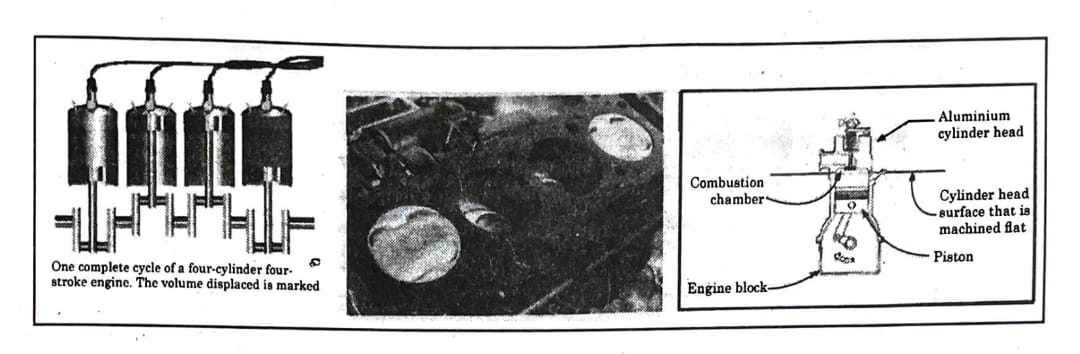
\includegraphics[height=7cm,width=12cm]{./figs/q1.png}
\caption{cylinder bore}
\label{fig:fig1}
\end{figure}
The cylinder bore in the form of circular cylinder open at the top is to be made from a metal sheet of area $75\pi cm^2$.\\Based on the above information, answer the following questions:
		  \begin{enumerate}
			  \item If the radius of cylinder is r cm and height is h cm, then write the volume V of cylinder in terms of radius r.
			  \item Find $\frac{dV}{dr}.$
			  \item \begin{enumerate}

					  \item Find the radius  of cylinder when its volume is maximum.
					  \item For maximum volume,$ h \ge r.$ State true or false and justify.
			  \end{enumerate}
		  \end{enumerate}
	  \item The use of electric vehicles will curb air pollution in the long run.
\figref{fig:Fig2}
		\begin{figure}[h!]
		\centering
		  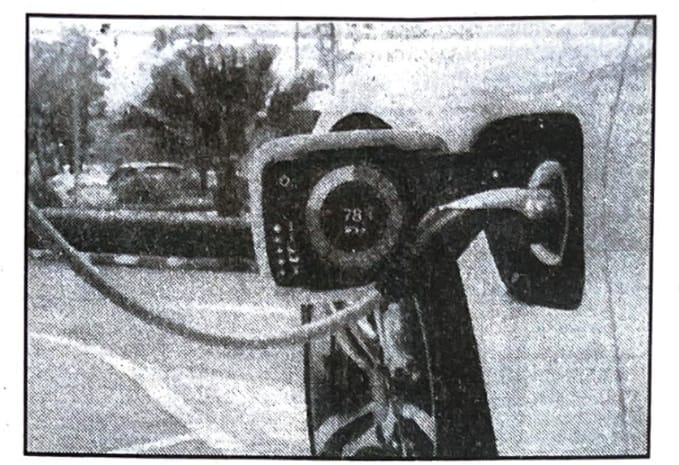
\includegraphics[height=7cm,width=11cm]{./figs/q3.png}
\caption{car}
\end{figure}
		  The use of electric vehicles is increasing every year and estimated electric vehicles in use at any time t is given by the function V:\\
	 \quad $V(t) = \frac{1}{5}t^3 - \frac{5}{2}t^2 + 25t - 2 $\\where t represents the time and t = 1, 2, 3.... corresponds to year 2001,2002, 2003,.....respectively.\\Based on the above information, answer the following questions:
		  \begin{enumerate}
			  \item Can the above function be used to estimate number of vehicles in the year 2000 ? Justify.
			  \item Prove that the function V(t) is an increasing function.
		  \end{enumerate}

 \end{enumerate}


\section{2022}
\subsection{12}
\input{2022/maths.tex}
\section{2021}
\subsection{10}
\input{2021/diff.tex}
\section{2021}
\subsection{12}
\input{2021/diffn.tex}
\section{2021}
\subsection{12}
\input{2021/differ.tex}
\section{2020}
\subsection{12}
\input{2020/diff.tex}
\section{2019}
\subsection{12}
\input{2019/differ_19.tex}
\input{2019/differ55.tex}
\input{2019/diff202.tex}
\input{2019/differ19d.tex}
\input{2019/diff203.tex}
\section{2018}
\subsection{12}
\input{2018/difh.tex}
\input{2018/diff6.tex}
\input{2018/diff8.tex}

\section{2017}
\subsection{10}

\subsection{12}
\input{2017/diff17.tex}

\section{2016}
\subsection{12}
\input{2016/diff.tex}
\input{2016/DIFF53 .tex}

\section{2015}
\subsection{12}
\input{2015/diff.tex}

\section{2022}
\subsection{12}
\begin{enumerate}
  \item If $\tan\brak{\frac{x+y}{x-y}}=k$, then $\frac{dy}{dx}$ is equal to
    \begin{enumerate}
        \item $ \frac{-y}{x} $
        \item $  \frac{y}{x} $ 
        \item $ \sec^2\brak{\frac{y}{x}}$ 
        \item $ -\sec^2\brak{\frac{y}{x}} $  
    \end{enumerate}
    \item \textbf{Assertion(A):} Maximum value of $(\cos^{-1} x)^2$ is $\pi^2$.\\
    \textbf{Reason(R):} Range of the principal value branch of $\cos^{-1}x$ is $\sbrak{\frac{-\pi}{2},\frac{\pi}{2}}$
    \item \begin{enumerate}
                \item If $ y= \sqrt{ax + b} $, then prove that $y\brak{\frac{d^2y}{dx^2}} + \brak{\frac{dy}{dx}}^2 = 0$
              \item If $f(x) = 
              \begin{cases}
              ax + b & \quad  0 \le x \leq 1\\
              2x^2 - x & \quad 1 \le x \le 2
              \end{cases}$ is a differentiable function in (0, 2), then find the values of a and b.
        \end{enumerate}
\item If the circumference of the circle is increasing at a constant rate , prove that the rate of change of area of the circle is directly proportional to its radius.
 \item Engine displacement is the measure of the cylinder volume swept by all pistons of a piston engine. The piston moves inside the cylinder bore.
		\figref{fig:fig1}
\begin{figure}[h!]
		\centering
		  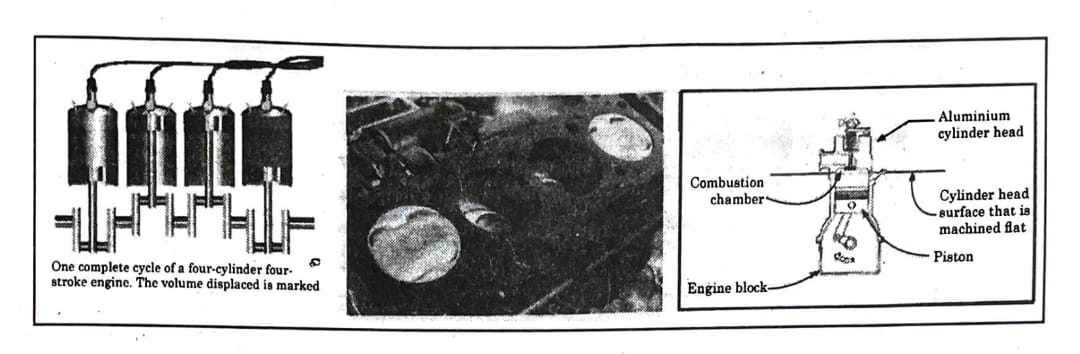
\includegraphics[height=7cm,width=12cm]{./figs/q1.png}
\caption{cylinder bore}
\label{fig:fig1}
\end{figure}
The cylinder bore in the form of circular cylinder open at the top is to be made from a metal sheet of area $75\pi cm^2$.\\Based on the above information, answer the following questions:
		  \begin{enumerate}
			  \item If the radius of cylinder is r cm and height is h cm, then write the volume V of cylinder in terms of radius r.
			  \item Find $\frac{dV}{dr}.$
			  \item \begin{enumerate}

					  \item Find the radius  of cylinder when its volume is maximum.
					  \item For maximum volume,$ h \ge r.$ State true or false and justify.
			  \end{enumerate}
		  \end{enumerate}
	  \item The use of electric vehicles will curb air pollution in the long run.
\figref{fig:Fig2}
		\begin{figure}[h!]
		\centering
		  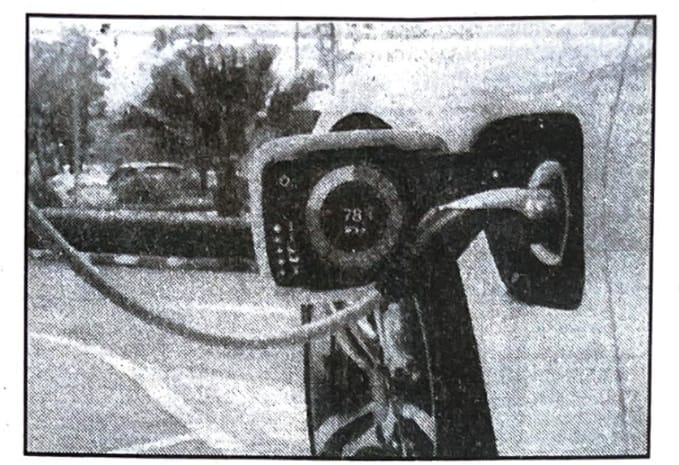
\includegraphics[height=7cm,width=11cm]{./figs/q3.png}
\caption{car}
\end{figure}
		  The use of electric vehicles is increasing every year and estimated electric vehicles in use at any time t is given by the function V:\\
	 \quad $V(t) = \frac{1}{5}t^3 - \frac{5}{2}t^2 + 25t - 2 $\\where t represents the time and t = 1, 2, 3.... corresponds to year 2001,2002, 2003,.....respectively.\\Based on the above information, answer the following questions:
		  \begin{enumerate}
			  \item Can the above function be used to estimate number of vehicles in the year 2000 ? Justify.
			  \item Prove that the function V(t) is an increasing function.
		  \end{enumerate}

 \end{enumerate}











\chapter{Integration}
\section{2023}
\subsection{12}
\input{2023/integration.tex}
\section{2022}
\subsection{12}
\begin{enumerate}
\item 
Integration:
\begin{align*}
\centering   
\int_{0}^{1} x^2 e^x \, dx
\end{align*}


\item 
Find the general solution for this differential equation:
\begin{align*}
\centering
\sec^2 x \tan y \, dx + \sec^2 y \tan x \, dy = 0
\end{align*}


\item 
If the area of the region bounded by the line $y = mx$ and the curve $x^2 = y$ is $\frac{32}{3}$ sq. units, then find the positive value of $m$ using integration.


\item 
 Find:
\begin{align*}
\centering
\int \frac{1}{e^x+1} \, dx
\end{align*}


\item 
Evaluate:
\begin{align*}
\int_{1}^{4}\cbrak{ \abs {x} + \abs{3-x}}dx
\end{align*}


\item 
Evaluate:
\begin{align*}
\centering
\int_{-3}^{3} \frac{x^4}{1+e^x} \, dx
\end{align*}


\item 
 Find the particular solution of the differential equation:
\begin{align*}
\centering
x\frac{dy}{dx} + y + \frac{1}{1+x^2} = 0
\end{align*}
given that $y(1) = 0$.


\item 
 Find the general solution of the differential equation:
\begin{align*}
\centering    
x(y^3+x^3) \, dy = (2y^4+5x^3y) \, dx
\end{align*}


\item 
Find:
\begin{align*}
\centering
\int \frac{dx}{\sqrt{4x-x^2}}
\end{align*}


\item 
Find the general solution of the following equation:
\begin{align*}
\centering
\frac{dy}{dx} = e^x - yx^2e^{-y}
\end{align*}


\item 
 Find:
\begin{align*}
\centering
\int e^x \sin(2x) \, dx
\end{align*}


\item 
 Find:
\begin{align*}
\centering
\int \frac{2x}{(x^2+1)(x^2+2)} \, dx
\end{align*}


\item 
Evaluate:
\begin{align*}
\centering
\int_{1}^{3} \frac{\sqrt{x}}{\sqrt{x}+\sqrt{4-x}} \, dx
\end{align*}


\item 
 Solve the following differential equations:
\begin{align*}
\centering
(y-\sin^2 x) \, dx + \tan(x) \, dy = 0
\end{align*}


\item 
 Find the general solution of the differential equation:
\begin{align*}
\centering
(x^3+y^3) \, dy = x^2y \, dx
\end{align*}


\item 
 Find:
\begin{align*}
\centering
\int \frac{1}{\sqrt{12+4x-x^2}} \, dx
\end{align*}


\item 
Find:
\begin{align*}
\centering
\int \frac{xe^x}{(x+4)^5} \, dx
\end{align*}


\item 
Find the general solution of the following differential equation:
\begin{align*}
\centering
(4+y^2)(3+\log x) \, dx + x \, dy = 0
\end{align*}


\item 
Evaluate:
\begin{align*}
\centering
\int_{0}^{\frac{\pi}{3}} \abs{ \cos(3x)}, dx
\end{align*}


\item 
 Find the general solution of the following differential equation:
\begin{align*}
\centering
2x e^{\frac{y}{x}} \, dy + (x-2y e^{\frac{y}{x}}) \, dx = 0
\end{align*}


\item 
 Find the particular solution of the differential equation:
\begin{align*}
\centering
(2x^2+y) \frac{dx}{dy} = x
\end{align*}
given that $y=2$ when $x=1$.


\item 
Find:
\begin{align*}
\centering
\int \frac{x^2+x+1}{(x+1)(x^2+4)} \, dx
\end{align*}


\item 
 Find the area bounded by the ellipse $x^2+4y^2=16$ and the ordinates $x=0$ and $x=2$, using integration.


\item 
 Find the area of the region $\{(x,y): x^2 \leq y \leq x\}$, using integration.


\item 
Find:
\begin{align*}
\centering
\int_{0}^{\frac{\pi}{2}} \frac{1}{1+\sqrt{\cot x}} \, dx
\end{align*}
 is equal to:
\begin{enumerate}
\item $\frac{\pi}{3}$
\item $\frac{\pi}{6}$
\item $\frac{\pi}{4}$
\item $\frac{\pi}{2}$
\end{enumerate}


\item 
Find:
\begin{align*}
\centering
\int \frac{(x+2)(x+2\log x)^3}{x} \, dx
\end{align*}


\item 
Find:
\begin{align*}
\centering
\int_{0}^{\frac{\pi}{2}} \log(\tan x) \, dx
\end{align*}


\item 
Find:
\begin{align*}
\centering
\int_{-1}^{2} \abs{x}\, dx
\end{align*}


\item 
Find:
\begin{align*}
\centering
\int\limits x^2 \log x. dx
\end{align*}


\item 
Find the general solution of the following differential equation :
\begin{align*}
\centering
\frac{dy}{dx}= (1+x)(1+y)
\end{align*}



\item 
Find the integrating factor for the following differential equation:
\begin{align*}
\centering
\frac{dy}{dx}+ y \cot x = 2x+x^2 \cot x (x \neq 0)
\end{align*}

 
\item 
Find:
\begin{align*}    
\centering
\int\limits\frac{x}{(x-1)^2(x+2)} dx
\end{align*}


\item 
Find the following differential equation :
\begin{align*}
\centering
x\cos \brak{\frac{y}{x}} \frac{dy}{dx}=y \cos \brak{\frac{y}{x}}+x 
\end{align*}

\item Find the sum of the order and the degree of the differential equation :
      $\brak{x+\frac{dx}{dy}}^2 = \brak{\frac{dy}{dx}}^2 + 1$ 
      \item  If $\frac{d}{dx}(x)$ = $\frac{\sec ^4 x}{\csc ^4 x}$ and 
      $F\brak{\frac{\pi}{4}}$ = $\frac{\pi}{4}$, then find $F(x)$
      
      \item Find : $\int \frac{\log x-3}{(\log x)^4}dx.$
      \item Find : $\int \frac{dx}{\sqrt{x}+\sqrt[3]{x}}.$
      \item Evaluate : $\int_{0}^{\pi/2}$ $ \frac{\cos x}{(1 + \sin x)(4 + \sin x)}dx$
      \item Evaluate : $\int_{0}^{\pi} \frac{x}{1 + \sin x}dx.$
      \item Using integration, find the area of the region enclosed by the curve $y = x^2$, the x-axis and the ordinates $x=-2$ and $x=1$.
      \item Using integration, find the area of the region enclosed by line $y = \sqrt{3x}$, semi-circle $y = \sqrt{4-x^2}$ and x-axis in first quadrant.
      \item Find the product of the order and the degree of the differential equation  
      $\frac{d}{dx}\brak{xy^2}\cdot \frac{dy}{dx}+y = 0$. 
      \item Find : $\int \frac{\sqrt{\cot x}}{\sin x \cos x} dx$
      \item Find : $\int \frac{1}{x(x^2 + 4)}dx$
      \item Evaluate : $\int_{0}^{1} \tan^{-1} xdx$
      \item Find : $\int \frac{2x}{x^2 + 3x + 2 } dx$
      \item Solve the following differential equation :
      $\left(1 + e^{y/x}\right)dy + e^{y/x} (1-\frac{y}{x})dx = 0$
      \item Evaluate : $\int_{0}^1 x(1-x)^n dx$
      \item Using integration, find the area of the smaller region enclosed the curve  $4x^2 + 4y^2 = 9$ and the line $2x + 2y = 3$
      \item If the area of the region bounded by the curve $y^2 = 4ax$ and the line $x = 4a$ is $\frac{256}{3}$ sq.units, then using integration, find the value of a, where $a > 0$.
      \item Find the general solution of the differential equation : $\frac{dy}{dx}=\cfrac{3e^{2x}+3e^{4x}}{e^x + e^{-x}}$
      \item Find : $\int \frac{dx}{x^2 - 6x + 13}$
      \item Find the particular solution of the differential equation  $x \frac{dy}{dx}-y = x^2 \cdot e^x$, given  $y(1) = 0$.
      \item Find the general solution of the differential equation $x\frac{dy}{dx}=y(\log y- \log x+1)$
      \item Evaluate : $\int_{-\pi/2}^{\pi/2} \brak{\sin \abs{x} + \cos \abs{x} }dx$
      \item Find : $\int \frac{x^2}{ (x^2 + 1)(3x^2 + 4)}dx$
      \item Evaluate : $\int_{-2}^1 \sqrt{5-4x-x^2}dx$
      \item Find the area of the region enclosed by the curves $y^2 = x$, $x = \frac{1}{4}$, $y = 0$ and $x = 1$, using integration.
      \item $\int \frac{\cos 8x + 1}{\tan 2x - \cot 2x} dx = \lambda \cos 8x + c $, then the value of $\lambda$ is 
      \begin{enumerate}
          \item  $\frac{1}{16}$
          \item  $\frac{1}{8}$
          \item  $-\frac{1}{16}$
          \item  $-\frac{1}{8}$
          
      \end{enumerate}
      \item $\int_{0}^1 \tan (\sin ^{-1}x) dx$ equals 
      \begin{enumerate}
          \item  2
          \item  0
          \item -1
          \item  1
      \end{enumerate}
      \item The integrating factor of the differential equation 
      $x\brak {\frac{dy}{dx}}-y= \log x$ is $\underline{\hspace{2cm}}$.
      \item Find the solution of the differential equation $\log \brak{\frac{dy}{dx}} = ax +by$
      \item Solve the following homogeneous differential equation : 
      $x \brak{\frac{dy}{dx}} = x + y$
      \item Evaluate $\int_{1}^3 (x^2 + 1 + e^x )dx$ as the limit of sums.
      \item If the area between the curves $x = y^2$  and $x = 4$ is divided into two equal parts by the line $x = a$, then find the value  of a using integration.
      \item Find : $\int \frac{x}{(x + 1 )^2 (x + 2)}dx$
      \item Evaluate : $\int_{0}^1 \frac{xe^x}{(x + 1)^2 } dx$
      \item Solve the following differential equation : $\brak {\frac{dy}{dx}} = e^{x+y} + x^2e^y$ 
      \item The supply function of  a commodity is $100p = (x+20)^2$. Find producer's surplus (PS), when the market price is \rupee 25.
      \item Find : $\int \frac{2x^2 + 1}{x^2 - 3x + 2}dx$
      \item In a certain culture of bacteria, the rate of increase of bacteria is proportional to the number present. It is found that there are $10,000$ bacteria at the end of $3$ hours and $40,000$ bacteria at the end of $5$ hours . determine the number of bacteria present int the beginning 




          \item Degree of differential equation $\sin x + \cos(\frac{\partial y}{\partial x})=y^2$ is
    \begin{enumerate}
        \item $2$
        \item $1$
        \item $not-defined$
        \item $0$
    \end{enumerate}
  \item  If $\frac{\partial f(x)}{\partial x}=2x+\frac{3}{x} $ and f(1)=1, then f(x) is
    \begin{enumerate}
        \item $x^2+3log|x|+1$
        \item $x^2+3log|x|$
        \item $2-\frac{3}{x^2}$
        \item $x^2+3log|x|-4$
    \end{enumerate}
    \item The integrating factor of the differential equation
     $(1-y^2)\frac{\partial x}{\partial y}+yx=ay,(-1<y<1) is$
    \begin{enumerate}
        \item $\frac{1}{y^2-1}$
        \item $\frac{1}{\sqrt{y^2-1}}$
        \item $\frac{1}{1-y^2}$
        \item $\frac{1}{\sqrt{1-y^2}}$
    \end{enumerate}
     \item Anti-derivative of $\frac{\tan x-1}{\tan x+1}$ with respect to x is:
    \begin{enumerate}
        \item $\sec^2\brak{\frac{\pi}{4}-x}+c$
        \item $-\sec^2\brak{\frac{\pi}{4}-x}+c$ 
        \item $log \lvert\sec\brak{\frac{\pi}{4}-x}\rvert+c$
        \item $-log \lvert\sec\brak{\frac{\pi}{4}-x}\rvert+c$ 
    \end{enumerate}
     \item Evaluate   $\int_{log {\sqrt 2}}^{log \sqrt{3}} \frac{1}{(e^x + e^{-x})(e^x - e^{-x})} dx$
     \item \begin{enumerate}
            \item Find the general solution of the differential equation:\\
	    $(xy-x^2)dy = y^2 dx$
 \item Find the general solution of the differential equation:\\ $(x^2 + 1)\frac{dy}{dx} + 2xy = \sqrt{x^2 + 4}$
        \end{enumerate}
	\item \begin{enumerate}
		    \item Evaluate $\int_{-1}^{1} \lvert x^4-x \rvert dx$
                    \item Find $\int \frac{\sin^{-1}x}{(1-x^2)^{3/2}} dx$
		    \end{enumerate}
		    \item Find $\int e^x \left(\frac{1-\sin x}{1-\cos x}\right) dx$
			    \item Using integration, find the area of triangle whose vertices are (-1, 1), (0, 5), (3, 2).
\end{enumerate}


\section{2021}
\subsection{12}
\input{2021/Int.tex}
\section{2020}
\subsection{12}
\input{2020/Int.tex}
\section{2019}
\subsection{12}
\input{2019/int_19.tex}
\input{2019/intr55.tex}
\input{2019/inte202.tex}
\input{2019/integ19d.tex}
\input{2019/int203.tex}
\section{2018}
\subsection{12}
\input{2018/inth.tex}
\input{2018/int6.tex}
\input{2018/int8.tex}

\section{2017}
\subsection{10}

\subsection{12}
\input{2017/inte17.tex}

\section{2016}
\subsection{12}
\input{2016/integrate.tex}
\input{2016/INTE53.tex}

\section{2015}
\subsection{12}
\input{2015/integrate.tex}


\chapter{Functions}
\section{2023}
\subsection{12}
\input{2023/Functions.tex}
\section{2022}
\subsection{12}
%\documentclass[12pt,-letter paper]{article}
%\usepackage{siunitx}
%\usepackage{setspace}
%\usepackage{gensymb}
%\usepackage{xcolor}
%\usepackage{caption}
%\usepackage{subcaption}
%\doublespacing
%\singlespacing
%\usepackage[none]{hyphenat}
%\usepackage{amssymb}
%\usepackage{relsize}
%\usepackage[cmex10]{amsmath}
%\usepackage{mathtools}
%\usepackage{amsmath}
%\usepackage{commath}
%\usepackage{amsthm}
%\interdisplaylinepenalty=2500
%\savesymbol{iint}
%\usepackage{txfonts}
%\restoresymbol{TXF}{iint}
%\usepackage{wasysym}
%\usepackage{amsthm}
%\usepackage{mathrsfs}
%\usepackage{txfonts}
%\let\vec\mathbf{}
%\usepackage{stfloats}
%\usepackage{float}
%\usepackage{cite}
%\usepackage{cases}
%\usepackage{subfig}
%\usepackage{xtab}
%\usepackage{longtable}
%\usepackage{multirow}
%\usepackage{algorithm}
%\usepackage{amssymb}
%\usepackage{algpseudocode}
%\usepackage{enumitem}
%\usepackage{mathtools}
%\usepackage{eenrc}
%\usepackage[framemethod=tikz]{mdframed}
%\usepackage{listings}
%\usepackage{listings}
%\usepackage[latin1]{inputenc}
%%\usepackage{color}{   
%%\usepackage{lscape}
%\usepackage{textcomp}
%\usepackage{titling}
%\usepackage{hyperref}
%\usepackage{fulbigskip}   
%\usepackage{tikz}
%\usepackage{graphicx}
%\lstsetframe=single,breaklines=t}
%\let\vec\mathbf{}
%\usepackage{enumitem}
%\usepackage{graphicx}
%\usepackage{siunitx}
%\let\vec\mathbf{}
%\usepackage{enumitem}
%\usepackage{graphicx}
%\usepackage{enumitem}
%\usepackage{tfrupee}
%\usepackage{amsmath}
%\usepackage{amssymb}
%\usepackage{mwe} % for blindtext and example-image-a in example
%\usepackage{wrapfig}
%\graphicspath{{figs/}}
%\providecommand{\mydet}[1]{\ensuremath{\begin{vmatrix}#1\end{vmatrix}}}
%\providecommand{\myvec}[1]{\ensuremath{\begin{bmatrix}#1\end{bmatrix}}}
%\providecommand{\cbrak}[1]{\ensuremath{\left\{#1\right\}}}
%\providecommand{\sbrak}[1]{\ensuremath{{}\left[#1\right]}}
%\providecommand{\brak}[1]{\ensuremath{\left(#1\right)}}


%\begin{document}
\begin{enumerate}
\item Let $R$ be the relation defined in $N$, as
$R = \cbrak{(x, y) : 2x + 3y = 15, x, y \in N}$, then $R$=  \cbrak{\underline{\hspace{1cm}},\underline{\hspace{1cm}}}.
\item If the function $f(x)=\begin{cases}\frac{k\cos{x}}{\pi - 2x}, & \text{if} x \neq \frac{\pi}{2}\\\text{2},&\text{if} x=\frac{\pi}{2}\end{cases}$  is continuous  at $x=\frac{\pi}{2}$, then the value of $k$ is {\underline{\hspace{1cm}}}.
\item Show that the relation $R$ in the set $\mathbb{R}$ of all real numbers,defined as $\mathbb{R}=\cbrak{(a, b) : a \leq b^2}$ is neither reflexive nor symmetric.
\item Find the value of $\tan^{-1}\sbrak{{2\cos}\brak{2 \sin^{-1}\brak{\frac{1}{2}}}}$
\item Let a function $f:\mathbb{R}-\cbrak{\frac{-4}{3}}\ \to \mathbb{R}$ be defined as $f(x)=\frac{4x}{3x+4}$.To show that $f$ is one-one function. Hence, find the inverse of the function $f:\mathbb{R}-\cbrak{\frac{-4}{3}} \ \to$ Range\hspace{0.25em} of $f$.
\item If $f:R\ \to R$ be given by $f(x)=\brak{3-x^3}^{1/3}$, then find $\brak{fof}\brak{x}$.
\item Let $W$ denote the set of words in the English dictionary. Define the relation $R$ by
$R={\brak{x,y}}\in W \times W$  such $x$ and $y$ have at least one letter in common. Show that this relation $R$ is reflexive and symmetric, but not transitive.
\item Find the inverse of the function $f(x)=\brak{\frac{4x}{3x+4}}$



\item The function $f(x)=x\lvert x \rvert is$
    \begin{enumerate}
        \item  continuous and differentiable at $x=0$
        \item  continuous but not differentiable at $x=0$
        \item  not continuous but differentiable at $x=0$
        \item neither continuous nor differentiable at $x=0$  
    \end{enumerate}
		\item \begin{enumerate}
         \item Evalauate $\sin^{-1}\brak{\sin \frac{3\pi}{4}} + \cos^{-1}\brak{\cos \pi } + \tan^{-1}(1)$.
         \item Draw the graph of $\cos^{-1} x$, where x $\in$ $\sbrak{-1, 0}$.Also, write its range.
     \end{enumerate}
	      \item A function $f: [-4, 4] \rightarrow [0, 4]$ is given by $f(x) = \sqrt{16 - x^2}$. Show that f is an onto function but not a one-one function. Further, find all possible values of 'a' for which $f(a) = \sqrt{7}.$
\end{enumerate}

%\end{document}

\section{2021}
\subsection{10}
\input{2021/assignment_10.tex}
\subsection{12}
\input{2021/assignment_12.tex}
\section{2020} 
\subsection{12} 
\input{2020/functions.tex}
\section{2019} 
\subsection{12}
\input{2019/functions_19.tex}
\input{2019/func55.tex}
\input{2019/func202.tex}
\input{2019/function19d.tex}
\input{2019/fun203.tex}
\section{2018} 
\subsection{12}
\input{2018/funh.tex}
\input{2018/fun6.tex}
\input{2018/rel8.tex}
\section{2017}
\subsection{10}

\subsection{12}
\input{2017/fun17.tex}

\section{2016}
\subsection{12}
\input{2016/func.tex}
\input{2016/FUN53.tex}




\chapter{Matrices}
\section{2020}
\subsection{10}
\input{2020/mat10.tex}
\section{2020}
\subsection{12}
\input{2020/mat12.tex}
\section{2022}
\subsection{10}
\input{2022/matrices10.tex}
\subsection{12}
\begin{enumerate}
\item If \mydet{3x & 3 & \\ 13 & x} = \mydet{4 & -2 \\ 8 & 5}, then the value of $x$ is :
	\begin{enumerate}
		\item $3$
		\item $\pm5$
		\item $25$
		\item $\pm1$
	\end{enumerate}
\item For $A= \myvec{\cos\alpha & -\sin\alpha \\ \sin\alpha & \cos\alpha}$, if $A + A' = O$, then the value of $\alpha$ is:
	\begin{enumerate}
		\item $\frac{\pi}{6}$
		\item $\frac{\pi}{3}$
		\item $\frac{\pi}{2}$
		\item $\pi$
	\end{enumerate}
\item For the matrix $A = \myvec{1&1&1\\1&2&-2\\2&-1&3}$, \\show that $A^3 -6A^2 + 5A +11I = 0$. Hence, find $A^{-1}$.
\item Using the properties of determinants, solve the following for $x$: 
	\begin{align}
		\mydet{x+3 & x+7 & x-1 \\ x+7 & x-1 & x+3 \\ x-1 & x+3 & x+7} = 0
	\end{align}
\item Find the value of $x$, if \mydet{5&3&-1\\-7&x&2\\9&6&-2}=0.
\item If $A= \myvec{4x&0\\2x&2x}$ and $A^{-1}=\myvec{1&0\\-1&2}$, then $x= \rule{2cm}{0.15mm}$.
\item If $A=\myvec{1&-1\\-1&1}$, then $A^2$ equals 
	\begin{enumerate}
		\item $\myvec{2&-2\\-2&2}$
		\item $\myvec{2&-2\\-2&-2}$
		\item $\myvec{-2&-2\\-2&2}$
		\item $\myvec{-2&2\\2&-2}$
	\end{enumerate}
\item The roots of the equation $\mydet{x&0&8\\4&1&3\\2&0&x}=0$ are
	\begin{enumerate}
		\item $-4,4$
		\item $2,-4$
		\item $2,4$
		\item $2,8$
	\end{enumerate}
\item A square matrix $A$ is said to be singular if \rule{2cm}{0.15mm}.
\item If $A= \myvec{3&-5\\2&0}$ and $B=\myvec{1&17\\0&-10}$, then $\mydet{AB}$= \rule{2cm}{0.15mm}.
\item if $\myvec{4&x+2\\2x-3&x+1}$ is symmetric matrix, then find the value of $x$.
\item If $A$ is a square matrix such that $A^2=A$, then find $(2+A)^3 -19A$.
\item For the matrix $A=\myvec{2&3\\-4&-6}$, verify the following:
	\begin{align}
		A(adj A) = (adj A)A= \mydet{A}I
	\end{align}
\item Using properties of determinants show that
	\begin{align}
		\mydet{1+a^2-b^2 & 2ab & -2b \\ 2ab & 1-a^2+b^2 & 2a \\ 2b & -2a & 1-a^2-b^2} = (1+a^2+b^2)
	\end{align}
\item Find the equation of the line join $A\brak{1, 3}$ and $B\brak{0, 0}$, using determinants. Also find $k$ if $D\brak{k,0}$ is a point such that the area of $\triangle ABD$ is $3$ square units.

\item If (a, b),(c, d),(e, f) are the vertices of $\triangle ABC$ and $\triangle$ denotes the area of $\triangle ABC$, then 
        ${\begin{vmatrix}
            a& c& e \\ b& d& f \\ 1& 1& 1  
        \end{vmatrix}} $ is equal to
    \begin{enumerate}
        \item $ 2\triangle^2 $
        \item $  4\triangle^2 $ 
        \item $  2\triangle $ 
        \item $ 4\triangle $ 
    \end{enumerate}
		\item If A is a ${2 \times 3}$ matrix such that AB and AB\' both are defined, then order of the matrix B is
    \begin{enumerate}
        \item $  2 \times 2  $
        \item $  2 \times 1 $ 
        \item $ 3 \times 2 $ 
        \item $  3 \times 3 $ 
    \end{enumerate}

    \item If $\begin{bmatrix} 2& 0 \\5& 4 \end{bmatrix}=P + Q$, where P is a symmetric and Q is a skew symmetric matrix, then Q is equal to
    \begin{enumerate}
        \item $ \begin{bmatrix} 2& \frac{5}{2}\\ \frac{5}{2}& 4 \end{bmatrix} $
        \item $ \begin{bmatrix} 0& \frac{-5}{2}\\ \frac{5}{2}& 0 \end{bmatrix} $ 
        \item $ \begin{bmatrix} 0& \frac{5}{2}\\ \frac{-5}{2}& 0 \end{bmatrix} $ 
        \item $  \begin{bmatrix} 2& \frac{-5}{2}\\ \frac{5}{2}& 4 \end{bmatrix} $ 
    \end{enumerate}
    \item If $\begin{bmatrix} 1& 2& 1\\ 2& 3& 1\\ 3& 1& 1 \end{bmatrix}$ is a non singular matrix and $a \in A$, then the set A is
    \begin{enumerate}
        \item $ \mathbb{R} $
        \item $ \{0\} $ 
        \item $  \{4\} $ 
        \item $ \mathbb{R} - \{4\} $ 
    \end{enumerate}
    \item If $A=\lvert kA \rvert$, where A is a square matrix of order 2, then sum of all possible values of k is
    \begin{enumerate}
        \item $  1 $
        \item $  -1 $ 
        \item $  2 $ 
        \item $  0 $ 
    \end{enumerate}
    \item \begin{enumerate}
		  \item If A = $\begin{bmatrix}
				  -3& -2& -4 \\ 2& 1& 2\\2& 1& 3
			  \end{bmatrix}$ and B = $\begin{bmatrix} 1& 2& 0\\ -2& -1& -2\\0& -1& 1\end{bmatrix}$, then find AB and use it to solve the following system of equations:\\
				  \begin{center}
					$  x - 2y = 3$\\
					  $2x - y - z = 2 $\\
					  $-2y + z = =3 $\\
				  \end{center}
			  \item If $f(\alpha) = \begin{bmatrix}
			  \cos \alpha& -\sin \alpha& 0\\\sin  \alpha& \cos \alpha& 0\\0& 0& 1  \end{bmatrix}$, then prove that $f(\alpha) \cdot f(-\beta) = f(\alpha - \beta)$
	\end{enumerate}

\end{enumerate}

\section{2023}
\subsection{10}
\input{2023/matrix_class_10.tex}
\subsection{12}
\input{2023/matrix_class_12.tex}
\section{2021}
\subsection{12}
\input{2021/matrix_12_2.tex}
\section{2021}
\subsection{12}
\input{2021/matrix_12_1.tex}
\subsection{10}
\input{2021/matrix_10.tex}
\section{2021}
\subsection{12}
\input{2021/matrix_12_3.tex}
\section{2019}
\subsection{12}
\input{2019/matrices_19.tex}
\input{2019/matr55.tex}
\input{2019/matr202.tex}
\input{2019/matrix19d.tex}
\input{2019/matr203.tex}


\section{2019}
\subsection{10}
\input{2019/matrrj.tex}

\section{2018}
\subsection{12}
\input{2018/math.tex}
\input{2018/mat6.tex}
\input{2018/mat8.tex}

\section{2017}
\subsection{10}

\subsection{12}
\input{2017/mat17.tex}


\section{2016}
\subsection{12}
\input{2016/mat.tex}
\input{2016/MATR53.tex}

\section{2015}
\subsection{12}
\input{2015/mat.tex}





\chapter{Trignometry}
\section{2019}
\subsection{10}
\input{2019/trignj.tex}
\section{2018}
\subsection{10}
\input{2018/trig22.tex}
\section{2017}
\subsection{10}
\input{2017/trig1.tex}


\section{2016}
\subsection{12}
\input{2016/Trigonometry.tex}
\input{2016/TRI53.tex}
\section{2015}
\subsection{10}
\input{2015/trigo.tex}
\section{2012}
\subsection{10}
\input{2012/trigonometry.tex}

\section{2011}
\subsection{10}
\input{2011/trignometry_psv.tex}
\input{2011/trignometry_ds.tex}

%\include{ch02} 
\backmatter
\appendix
\iffalse
\chapter{Conic Lines}
\section{Pair of Straight Lines}
%
\input{quad/pair.tex}
\section{Intersection of Conics}
\input{quadlines/inter.tex}
\section{ Chords of a Conic}
\input{quadlines/chord.tex}
\section{ Tangent and Normal}
\input{quadlines/tangent.tex}
\fi
%\chapter{Proofs}
%   \section{}
%\input{apps/defs.tex}

%  \section{}
%\input{apps/parab.tex}
%  \section{}
%\input{apps/nonparab.tex}
%		\section{}
%\input{apps/params.tex}
\latexprintindex

\end{document}

 
\section{Examples}
\subsection{Loney}
\input{examples/loney.tex}
\subsection{Miscellaneous}
\input{examples/misc.tex}
%
%%\section*{Disclosure Statement}
%%The authors report there are no competing interests to declare.
%%
%%
%%
%%  
%%%All the results related to conics are summarized in 
%%%Table \ref{table:conics}.  
%%%\begin{table*}[!t]
%%%\centering
%%%\input{conics.tex}
%%%%\input{./figs/conics.tex}
%%%\caption{$\vec{x}^{\top}\vec{V}\vec{x}+2\vec{u}^{\top}\vec{x}+f = 0$  can be expressed in the above standard form for various conics. $\vec{c}$ represents the centre/vertex of the conic. $\vec{q}$ is/are the point(s) of contact for the tangent(s). }
%%%\label{table:conics}
%%%\end{table*}
%%%\begin{verbatim}
%%\bibliographystyle{tfs}
%%%\bibliography{interacttfssample}
%%\bibliography{school}
%%\end{verbatim}
%% included where the list of references is to appear, where \texttt{tfs.bst} is the name of the \textsc{Bib}\TeX\ bibliography style file for Taylor \& Francis' Reference Style S and \texttt{interacttfssample.bib} is the bibliographic database included with the \textsf{Interact}-TFS \LaTeX\ bundle (to be replaced with the name of your own .bib file). \LaTeX/\textsc{Bib}\TeX\ will extract from your .bib file only those references that are cited in your .tex file and list them in the References section.
%
%% Please include a copy of your .bib file and/or the final generated .bbl file among your source files if your .tex file does not contain a reference list in a \texttt{thebibliography} environment.
%

  % \section{Appendices}
  % \appendix

\appendices
